\documentclass{article}
\usepackage{geometry}
\geometry{a4paper,top=2cm,bottom=2cm,left=1.5cm,right=1.5cm,%
	heightrounded,bindingoffset=5mm} %sistemiamo questi per decidere i bordi
\usepackage[utf8]{inputenc}
\usepackage{wrapfig}
\usepackage{float}
\usepackage{caption}
\usepackage[cc]{titlepic}
\usepackage{graphicx}
\usepackage{natbib}
\usepackage{makecell}
\usepackage{graphicx}
\usepackage{multirow}
\usepackage[table,xcdraw]{xcolor}
\usepackage{color, colortbl}
\definecolor{Gray}{gray}{0.9}
\definecolor{LightCyan}{rgb}{0.88,1,1}
\usepackage[first=0,last=9]{lcg}
\newcommand{\ra}{\rand0.\arabic{rand}}

\newcommand{\specialcell}[2][c]{%
	\begin{tabular}[#1]{@{}c@{}}#2\end{tabular}}


\begin{document}
	
	\begin{titlepage}
		\centering
		
\includegraphics[width=0.80\textwidth]{marchio.jpg}\par\vspace{2cm}
		{\scshape\LARGE Data Mining Report \par}
		\vspace{1cm}
		{\scshape\Large Group 12 \\ \par}
		\vspace{1cm}
		{\huge\bfseries Analysis of car auctions\par}
		\vspace{2cm}
		{\Large\ Lorenzo Bellomo \\ Andrea Bruno \\ Marta Scalisi \\ Chiara Spampinato\par}
		\vspace{4cm}
		{\Large\ January 2020\par}
	\end{titlepage}
	
	
	
	
	\section{Data Understanding}
	The data set contains information about car auctions. The majority of attributes give us information about vehicles. 
	In this section, we'll explain how we studied our data, evaluated the quality of them, how we fixed any missing values (invalid or misleading), in order to gain general insights about the data that would potentially be helpful for the complete analysis.
	
	\subsection{Data Semantics}
	\label{sec:dataSemantics}
	The semantic meaning of the most important (in our opinion) variables in the dataset are described in the following, while the remaining columns are not described either because their meaning is too obvious or because its discussion is delayed to the following sections.\begin{itemize}
		\item \emph{RefId}: attribute which defines an unique ID number assigned to each vehicle;
		\item \emph{Auction}: categorical attribute which defines three different auction providers (Manheim, Adesa, other);
		\item \emph{Make}: categorical attribute which gives us the name of the production company of the vehicle;
		\item \emph{VehOdo}: numerical discrete attribute that points out the mileage;
		\item \emph{VehBCost}: continuous numerical attribute indicating the purchase price auction;
		\item \emph{MMRA}: numerical attributes that define acquisition price of the vehicles, divided into:
		\begin{itemize}
			\item average condition price at time of purchase 
			\item above average condition price at time of purchase
			\item average condition price at time of purchase in the retail market
			\item above average condition price at time of purchase in the retail market 
		\end{itemize}
		\item \emph{MMRC}: numerical attributes that define the current price of the vehicles, divided into:
		\begin{itemize}
			\item average condition price as of current day 
			\item above condition price as of current day
			\item above average condition price as of current day
			\item above average condition  price as of current day in the retail market
		\end{itemize}
		\item \emph{WarrantyCost}: variable expressing cost of the warranty for the car at the time of the auction;
		\item \emph{IsBadBuy}: this is our target variable, and it expresses if the car was a good deal or not.
	\end{itemize}
	
	Furthermore, analyzing all the attributes there are two of them, Acquisition Type and Kickdate, which aren't in the dataset even though they are present in the dictionary.
	
	
	\subsection{Variables Transformation and elimination of redundant variables}
	
	We decided to split the attributes \emph{Model} and \emph{SubModel}, because, within them, too much information was contained. As a result, we use this information to create five different attributes:
	\begin{itemize}
		\item \emph{Engine Liters}: this information was in both the Model and SubModel columns, usually in the form of a float number and a L (i.e. 2.7L);
		\item \emph{NumCylinders}: this information was also present in both variables (i.e. V4, V-8, I4\dots);
		\item \emph{4X4}, four-wheel drive;
		\item \emph{WheelDrive}, other drive wheel configurations (i.e. 2WD, 4WD\dots); 
		\item \emph{NumDoors}, the number of the doors in a car (i.e. 5D);
	\end{itemize}
	The information contained in the five new attributes is not very interesting in itself, but with this approach we were able to "clean" the both columns from their meta-information. Taking as example the Model column, we were able to go from over 1000 unique models in the original data set to just around 200 without loss of information. 
	
	We also created four different attributes in order to separate the information contained in the variable \emph{PurchDate} into PurchYear, PurchMonth, PurchDay and PurchWeekDay (which is the working day of acquisition, like Monday, Tuesday\dots).
	
	For the sake of simplicity, from now on, the 8 MMR variables will be addressed with an abbreviation. For example, MMRAcquisitionRetailAveragePrice becomes ARAP, MMRCurrentAuctionCleanPrice becomes CACP, and so on.
	
	
	\begin{figure}[H]
		\centering
		{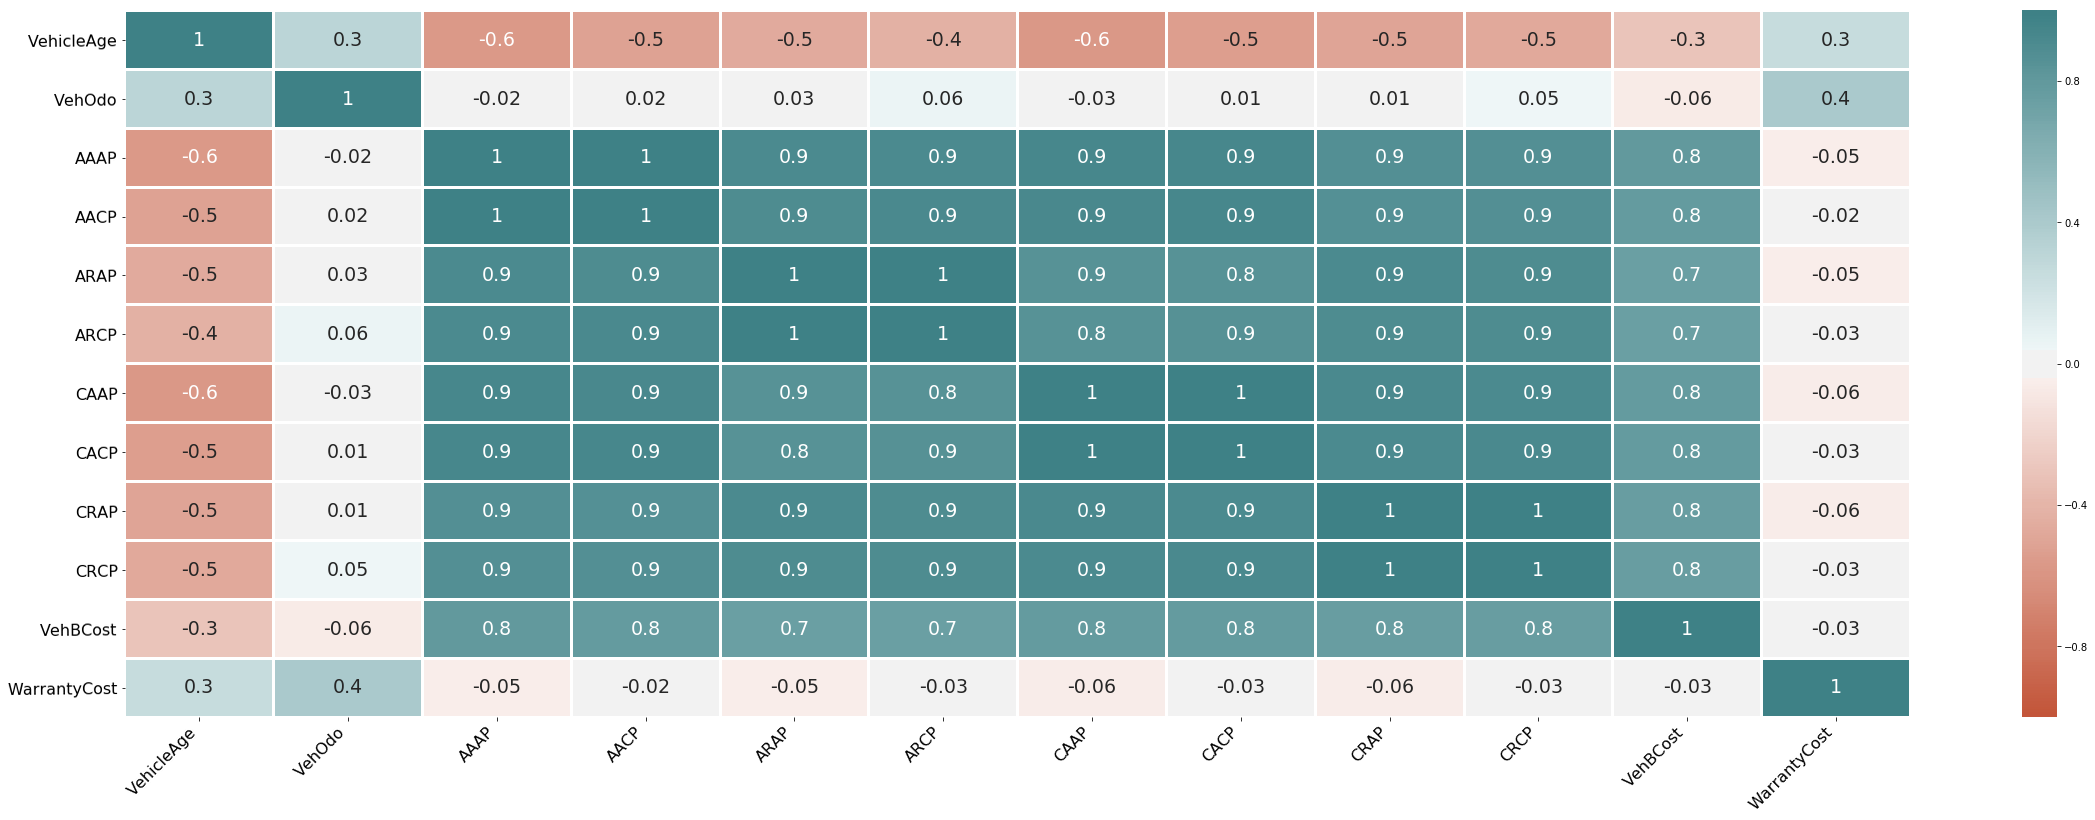
\includegraphics[width=\textwidth, keepaspectratio]{corr.png}}
		\caption{{ Correlation matrix }}
		\label{fig:corr}
	\end{figure}
	
	
	Finally, analyzing the correlation matrix (shown in the figure\ref {fig:corr},) of all the continuous attributes we can see that the 8 MMR attributes are strongly correlated (close to 0.9). Therefore, we reduced them into two attributes by using the algorithm PCA used to reduce the dimensionality of the data. We created 2 variables from the original 8, namely PCA1 and PCA2. The first one became the most correlated to the original prices, while the second one had a lower correlation and mainly expressed the variance between different attributes.\\
	However, for the sake of clarity, we used PCA1 and PCA2 only in section \ref{sec:classification}, when dealing with classification. We instead decided to use one candidate price (MMRAcquisitionAuctionAveragePrice, or AAAP for short) in section \ref{sec:patternmining} and section \ref{sec:clustering} when describing Pattern Mining and Clustering, in order to have clearer semantics regarding car prices. 
	The discussion regarding the distribution of MMR attributes and PCA ones is delayed to section \ref{sec:attrDistr}.
	
	
	\subsection{Assessing data quality}
	
	In order to assess the quality of data, we performed some variable wise consistency checks (for example on VehYear, VehicleAge, VehOdo, WarrantyCost), but we did not find any notable error. However, we found a lot of 0 values for the 8 MMR prices (in addition to its missing values), and we also identified one clear outlier in the VehBCost column, with this car having been sold at 10\$. We then decided to drop this row. \\
	Outlier wise, we found that the MMR prices were usually coherent with respect to the VehBCost attribute, so we decided to keep in the data set all the other rows. In this, we also kept a lot of very high-cost cars, but we could not label these cars as outliers, as we thought that this behavior is to be expected.
	
	\begin{figure}[H]
		\centering
		{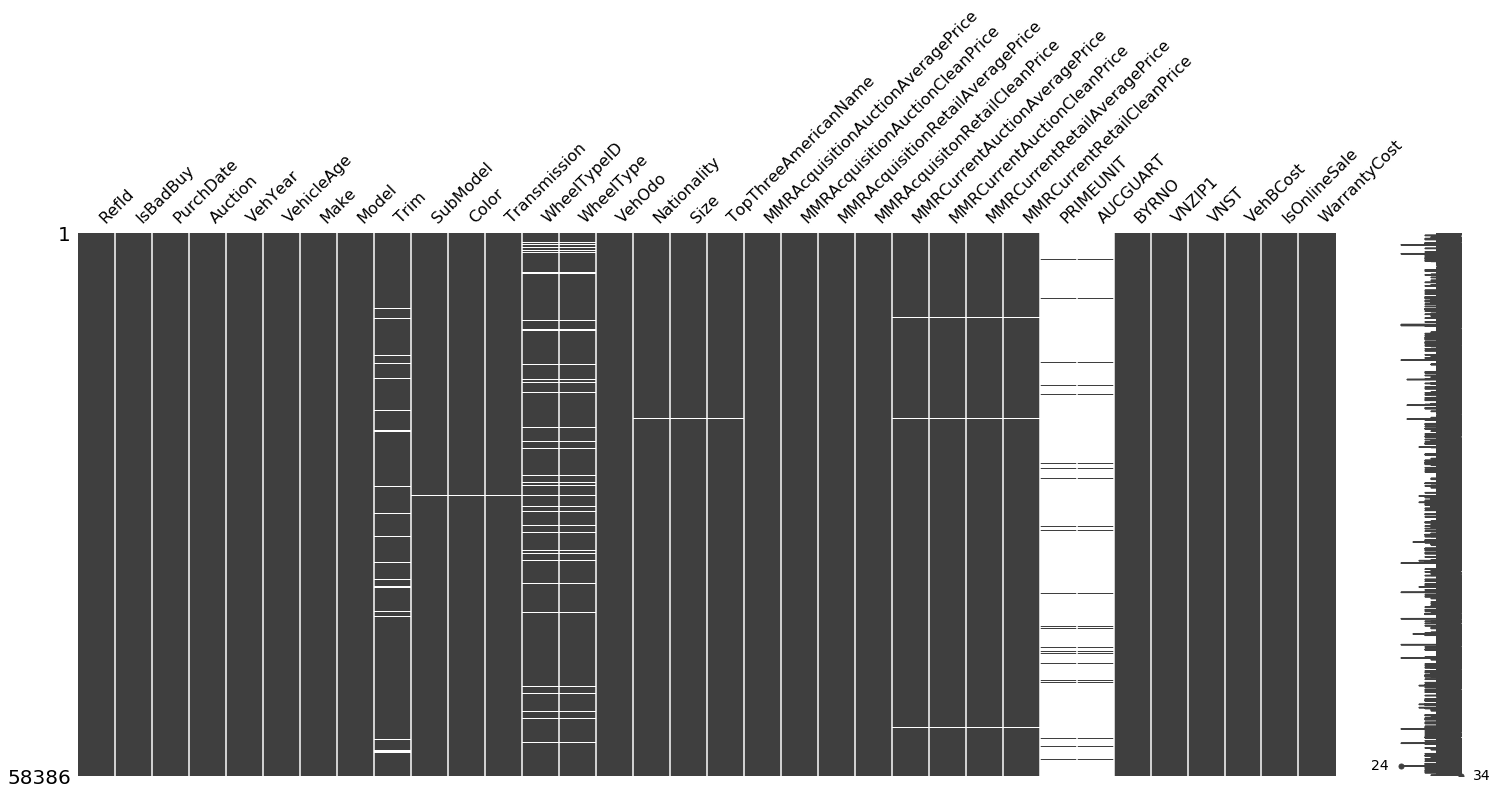
\includegraphics[width=\textwidth, height=.8\textheight, keepaspectratio]{missingv.png}}
		\caption{{ Missing values }}
		\label{fig:missingval}
	\end{figure}
	
	By looking at figure \ref{fig:missingval} it is possible to see the missing value of our dataset (identified by the white lines). The attributes PRIMEUNIT and AUCGUART have too many missing values, so we decide to discard and not use them.\\
	
	
	Analyzing the others, we chose to correct the variables Trim, Liters, Cylinders, Transmission with the algorithm MICE (Multiple Imputation by Chained Equations).
	
	
	
	\subsection{Attributes Distribution}
	\label{sec:attrDistr}
	In this section, we will analyze the distribution of some particular attributes, showing interesting statistic plots.
	
	The first thing to note is that the target variable (IsBadBuy), is highly imbalanced. Good buys are $87\sim88 \%$ of the population, while the remaining $12\sim13 \%$ are bad buys.
	
	In the plot shown in figure \ref{fig:mmr}, we show the distribution of the 8 numerical attributes which point out the different prices of Vehicle as we explained in the first part of Data Semantics (section \ref{sec:dataSemantics}). 
	\begin{figure}[H]
		\centering
		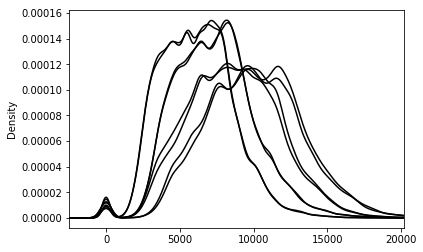
\includegraphics[width=.4\textwidth]{index}\hfill
		\includegraphics[width=.4\textwidth]{PCA1}
		\caption{Distribution of 8 MMR prices and of PCA1}
		\label{fig:mmr}
	\end{figure}
	
	We are able to notice that MMR attributes are very correlated, but the correlation is ever higher when considering them pairwise (when considering clean price and average price together). \\
	We are also able to notice that, before variable cleaning, there is a very high peak corresponding to the 0. This peak is no longer present in PCA1, as before applying the algorithm we considered those 0s as missing values and imputed them. 
	
	\begin{figure}[H]
		\centering
		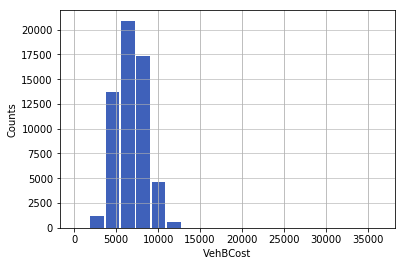
\includegraphics[width=.4\textwidth]{hist}\hfill
		\caption{Distribution of the attribute VehBCost}
	\end{figure}
	Analyzing the attribute \emph{VehBCost}, we can observe that Vehicles are usually sold for a price between 6000 and 7000, and a very low percentage of cars is sold above 11000 or below 5000 USD. 
	
	
	\begin{figure}[H]
		\centering
		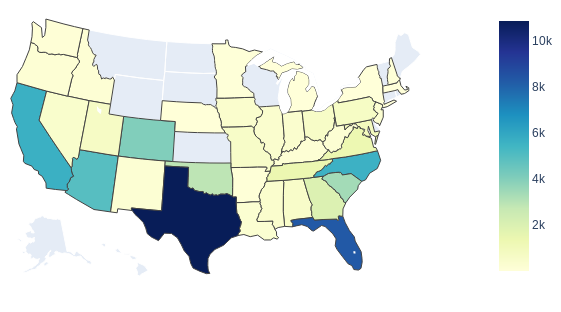
\includegraphics[width=.6\textwidth, height=.6\textheight, keepaspectratio]{newplot.png}
		\caption{{ Distribution of the attribute VSNT}}
	\end{figure}
	
	
	For the attribute \emph{VSNT} we decide to plot the distribution on a map of the United States. By looking at the figure, it is possible to see that the major number of auctions is done in Texas (18800), followed by Florida (8317) and California (5673). On the other hand, the state with lower auctions is New York (4). Furthermore, there are no auctions in Montana, Wyoming, North Dakota, South Dakota, Kansas, Wisconsin, Maine, Vermont, Rhode Island and Connecticut.
	\begin{figure}[H]
		\centering
		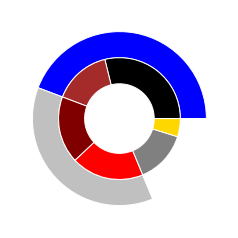
\includegraphics[width=.4\textwidth]{color.png}
		\caption{Distribution of the attribute Color}
		\label{fig:color}
	\end{figure}
	
	
	As far as it concerns the attribute \emph{Color} (figure \ref{fig:color}, it is not surprising that the most common colors are blue, silver and white.
	
	
	By analyzing also the distribution of the variable IsBadBuy in figure \ref{fig:badbuys}, plotted with respect to WarrantyCost and VehOdo on the left, and with respect to WheelType on the right, we can notice a few different things. Regarding the left image, bad purchases are more frequent in less dense areas. Regarding the image on the right, we are able to notice that, whenever WheelType information is lacking, the number of bad buys is huge with respect to the variable distribution (corresponding to the column labeled as \emph{Unknown}).
	
	\begin{figure}[H]
		\centering
		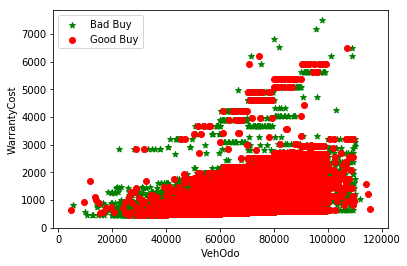
\includegraphics[width=.49\textwidth, keepaspectratio]{badbuys}
		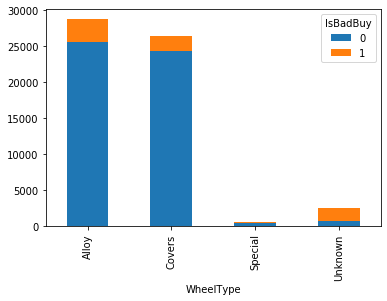
\includegraphics[width=.41\textwidth, keepaspectratio]{wheeltype}
		\caption{IsBadBuy distribution with respect to VehOdo and VehBCost}
		\label{fig:badbuys}
	\end{figure}
	
	
	
	\section{Clustering}
	\label{sec:clustering}
	In this section we describe the three Clustering algorithms applied to the data set (KMeans, DBScan and Hierarchical), and we describe the results
	
	\subsection{Function Selection}
	In K-means we tried to use both the \emph{MinMax} scaler and the standard \emph{z} scaler, observing that the clustering results were very similar. In the end, we decided to use the MinMax one.
	In DBScan and Hierarchical we decided to adopt the Standard one because it gave us slightly better results.
	
	\subsection{KMeans}
	The following sections discuss the analysis of the results of KMeans clustering algorithm.
	
	\subsection{Attributes' selection}
	Considering that our dataset contains information about car auctions, we opt to study characteristics about cars, like how many kilometers the car has done (\textbf{VehOdo}), the auction selling price for the car (\textbf{VehBCost}), the cost of repairing or replacing previously sold products (\textbf{WarrantyCost}) and some samples of the different prices (\textbf{AAAP, ARAP}).
	
	We created 5 Dataframes with these attributes in order to study which was the best combination of them.
	
	\begin{table}[H]
		\centering
		\begin{tabular}{c|ccccccc}
			\hline
			& Attributes set \\
			\hline
			\rowcolor{Gray}
			1 & 'VehOdo' ,  'VehBCost',  'AAAP' \\
			2 & 'WarrantyCost' , 'VehBCost' ,  'AAAP'  \\
			\rowcolor{Gray}
			3 & 'AAAP' ,  'ARAP' ,  'VehBCost' \\
			4 & 'WarrantyCost' ,  'VehOdo' ,  'VehBCost'  \\
			\rowcolor{Gray}
			5 & 'WarrantyCost' ,  'AAAP' , 'VehOdo' \\
			\hline
		\end{tabular}
	\end{table}
	
	
	\subsubsection{Identification of best k}
	
	
	In order to pick the best parameter k for K-Means, we made use of the Knee method by computing the SSE for K $\in$ [2,16]. The best SSE was obtained in the Data Frame 3, which was originally chosen for his highest correlation among the attributes.
	
	However, when we tried plotting the data, we did not obtain any interesting information in order to better interpreter the data behaviour. We then decided to give up the best SSE by choosing the Data Frame 4 which has a lower SSE but semantically more interesting results.
	
	
	\begin{figure}[H]
		\centering
		\includegraphics[width=.49\textwidth]{cattura}\hfill
		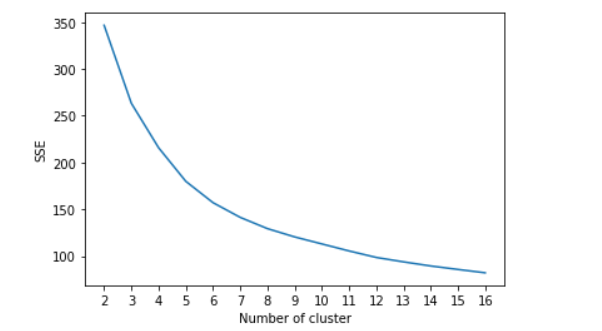
\includegraphics[width=.49\textwidth]{SSE2}\hfill
		\caption{Plot SSE of Attribute set 3 (left) and 4 (right).}
		\label{fig:KmeansSSE}
	\end{figure}
	We noticed that the SSE curves for the 5 data frames share a strong similarity (same curvature, but different SSE). Their behaviour is very similar to the ones shown in figure \ref{fig:KmeansSSE}, and we found, using the \emph{knee method}, that the best attribute \emph{k} for all the data frames was 6. All the values collected for the the different data frames are shown in table \ref{tab:SSESilu}. In particular, the lowest SSE is by far the one of data frame 3. \\However, we decided to discard this result since the 6 clusters found by the algorithm were basically groups of cars in different price ranges. We decided that the best clustering, both semantically and parameter wise, was the DF4 one (taking in consideration 'WarrantyCost', 'VehOdo' and 'VehBCost').
	
	\begin{table}[H]
		\centering
		\begin{tabular}{c|ccccccc}
			\hline
			&  Best k & SSE& Silhouette \\
			\hline
			\rowcolor{Gray}
			DF1 & 6 & 106.0 & 0.309 \\
			DF2 & 6 & 90.0 & 0.307  \\
			\rowcolor{Gray}
			DF3 & 6 & 40.0 & 0.294 \\
			DF4 & 6 & 157.0 & 0.287  \\
			\rowcolor{Gray}
			DF5 & 6 & 184.0\textbf & 0.278 \\
			\hline
		\end{tabular}
		\caption{{ Summary of the SSE, Silhouette and k values obtained for all the Attribute sets with K-means}}
		\label{tab:SSESilu}
	\end{table}
	
	
	\subsubsection{Description of the best clustering}
	\label{sec:clusterdescr}
	The following descriptions refer to the results of the clustering that were proposed as the best in previous section. Every result is presented with its centroid, that describes the core point of the cluster, and a textual interpretation of the kind of cars that are present in those clusters. 
	The centroids coordinates are expressed like this:  
	$$ \mathbf{centroid} = (\mathbf{VehBCost}, \mathbf{WarrantyCost}, \mathbf{VehOdo}) $$
	In figure \ref{fig:centroid} the clustering results are shown plotted in 2 dimensions (WarrantyCost and VehOdo). The plot does not show the third dimension (VehBCost) because, from the results, this latter one results the least important dimension (as it will be evident from the centroids shown when describing the clusters).
	The figure also shows the cluster centroids with a star on the plot. 
	
	\begin{figure}[H]
		\centering
		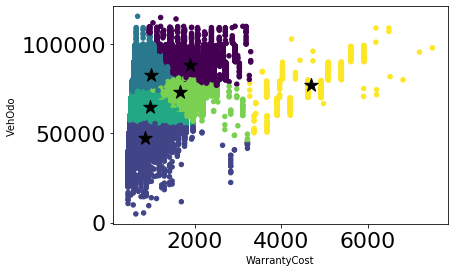
\includegraphics[width=.6\textwidth, keepaspectratio]{centroid}
		\caption{{Clusters plotted with WarrantyCost and VehOdo}}
		\label{fig:centroid}
	\end{figure}
	
	
	The clusters descriptions for figure \ref{fig:centroid} are:
	\begin{enumerate}
		\item $\mathbf{centroid}: (6\,500,  1\,900,  88\,000)$: cars with very high odometer reading and pretty high warranty cost (purple cluster). Those cars are sold for a price which is in line with the mean of the prices.
		\item $\mathbf{centroid}: (6\,800,  850,  48\,000)$: cars which are pretty new , with low  reading and low warranty cost (light blue cluster). As expected their cost is slightly above average.
		\item $\mathbf{centroid}: (6\,400,  1\,000,  83\,000)$: cars with high odometer reading but low warranty cost (azure cluster). Those cars are probably considered to be solid (low outage risk) even after years of use, and are sold at a normal price.
		\item $\mathbf{centroid}: (6\,700,  1\,000,  65\,000)$: cars with low warranty cost and average odometer (aquamarine cluster). There is not much to say about this cluster, as it represents the average car.
		\item $\mathbf{centroid}: (7\,300,  1\,700,  73\,000)$: Cars with high warranty cost, but average odometer reading (green cluster). This is one of the more interesting cluster, as it shows that relatively high risk cars are sold at a price which is higher than expected (considering high warranty cost as a sign of risk).
		\item $\mathbf{centroid}: (5\,300,  4\,700,  77\,000)$: Exceptionally high warranty cost, high odometer reading (yellow cluster). This cluster is the least populated one, and the most sparse one. It homes those very risky buys, and in addition to that, cars in this cluster are also pretty dated. They are sold, as expected, at a very low price. 
	\end{enumerate}
	Given these outcomes, we tried to understand if bad buys were located mainly in one of those clusters. By plotting this information in figure \ref{fig:clusterbuy}, we noticed that cluster 2 (new cars with low odometer reading), has the least amount of bad buys.
	\begin{figure}[H]
		\centering
		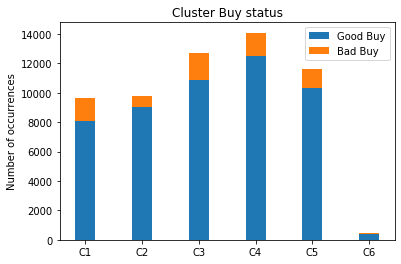
\includegraphics[width=.5\textwidth, keepaspectratio]{clusterbuy}
		\caption{{Distribution of IsBadBuy with respect to the 6 clusters found}}
		\label{fig:clusterbuy}
	\end{figure}
	
	
	
	
	\subsection{DB Scan}
	In this section, we explain the approach used to generate clusters with DBscan algorithm.
	
	\subsubsection{Attributes and distance function}
	
	We decided, following the same reasoning we used for \emph{KMeans}, to attempt clustering over the same set of attributes. We also decided to use Euclidean distance, and Z-Score scaling for the data frame.\\
	The results shown in the following sections are only relative to the data frame with columns 'VehOdo', 'VehBCost' and 'WarrantyCost' (the same data frame used for KMeans). Other possible attributes choices did not change much the final result, so we decided that using the same attributes allows us to more easily see the difference between the two algorithms.
	
	\subsubsection{Study of the clustering parameters}
	In order to choose the right $\epsilon$ and $\mathbf{min points}$, we adopted the knee method by plotting the distance to the \emph{k-th} nearest neighbour, where k was taken from [32, 64, 128, 256, 512]. The resulting curves, shown in figure \ref{fig:kth}, were used to select the right epsilon for attempting the clustering with DB-Scan. 
	
	\begin{figure}[H]
		\centering
		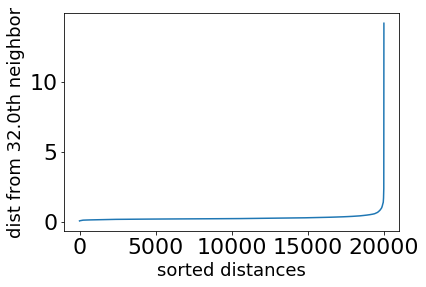
\includegraphics[width=.32\textwidth]{a32}\hfill
		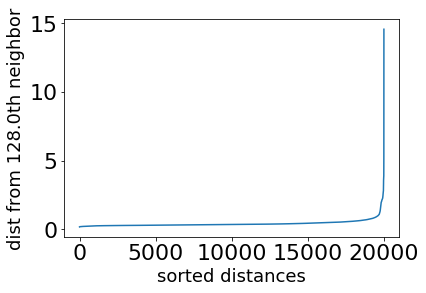
\includegraphics[width=.32\textwidth]{a128}\hfill
		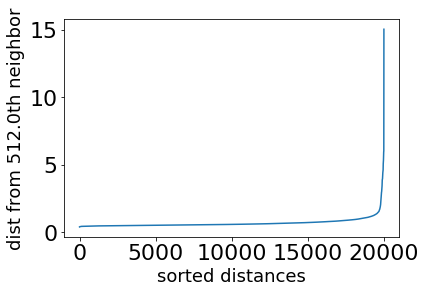
\includegraphics[width=.32\textwidth]{a512}
		\caption{k-th neighbour distance, with k = 32, k = 128, k = 512}
		\label{fig:kth}
	\end{figure}
	
	Given those plots, we chose epsilon as shown in table \ref{tab:kth}.
	It is important to know, however, that this approach failed for reasons described in section \ref{sec:dbscaneval}, so another set of attributes with more interesting results is shown in table \ref{tab:dbscan}. Those values were found by brute force, by attempting, for all k shown in the list before, $\epsilon = 0.1, 0.11, 0.12\dots 0.8$, and visually inspecting the results.\\
	
	\begin{table}
		\parbox{.45\linewidth}{
			\centering
			\begin{tabular}{c|c}
				\hline
				min points & $\epsilon$\\
				\hline
				\rowcolor{Gray}
				32 & 0.75 \\
				64 & 0.95 \\
				\rowcolor{Gray}
				128 & 1.22 \\
				256 & 1.36 \\
				\rowcolor{Gray}
				512 & 1.64 \\
				\hline
			\end{tabular}
			\caption{K-th nearest neighbours parameters}
			\label{tab:kth}
		}
		\hfill
		\parbox{.45\linewidth}{
			\centering
			\begin{tabular}{c|c}
				\hline
				min points & $\epsilon$\\
				\hline
				\rowcolor{Gray}
				32 & 0.17 \\
				64 & 0.22 \\
				\rowcolor{Gray}
				128 & 0.29 \\
				256 & 0.38 \\
				\rowcolor{Gray}
				512 & 0.48 \\
				\hline
			\end{tabular}
			\caption{Manually found parameters}
			\label{tab:dbscan}
		}
	\end{table}
	
	\subsubsection{Characterization and interpretation of the obtained clusters}
	\label{sec:dbscaneval}
	First, we are going to analyze the results with parameters shown in table \ref{tab:kth}. The result was that of a single cluster, containing all the points in the data set, with the exception of $\sim 100$ elements, which were labeled as noise points. This is because the data forms one big cloud of points, with different density distribution inside. This kind of behaviour represents the conditions under which DB scan performs worst, and this is the reason why the \emph{k-th} neighbour distance approach failed. \\
	We then decided to try and find the most dense areas in the data set, by manually checking a lot of configurations. This approach, however, does not find cluster, but it only finds highly populated areas in the data set. 
	The best results were found when the number of noise points was close to half the total amount in the data set. Those results correspond to the ones found with the parameters shown in table \ref{tab:dbscan} and some example of such clustering is shown in figure \ref{fig:dbscan}.
	
	\begin{figure}[H] 
		\centering
		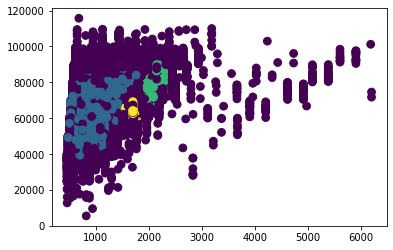
\includegraphics[width=.48\textwidth]{cazzo}\hfill
		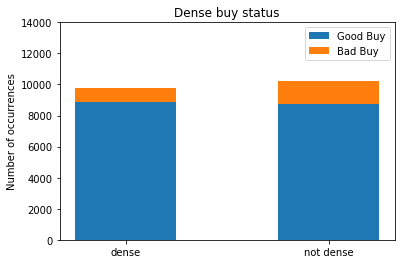
\includegraphics[width=.49\textwidth]{bigboi}\hfill
		\caption{DBScan clustering results with $\mathbf{minpoints} = 256$ and $\epsilon = 0.38$. Purple colors are noise points}
		\label{fig:dbscan}
	\end{figure}
	
	We realised that most of the cars sold have $50\,000 \sim 70\,000$ odometer reading when sold, and denser areas have slightly less bad buys overall. \\
	Having said that, DBscan is the algorithm that performs the worst on this data set.
	
	\subsection{Hierarchical Clustering}
	In this section, we explain the approach used to generate clusters with Hierarchical algorithm.
	\subsubsection{Attribute Choices}
	We decided to perform clustering on the following attributes set:
	\begin{enumerate}
		\item 'VehOdo', 'VehBCost', 'AAAP'
		\item 'WarrantyCost', 'VehBCost', 'VehOdo'
	\end{enumerate}
	
	\subsubsection{Algorithms and Dendrograms}
	\label{sec:hier}
	We decided to perform clustering with Euclidean and Manhattan distance as metrics, and to perform, for each of those metrics ward, single, complete and average linkages (with the exception of manhattan distance with ward linkage, since it is not allowed).\\
	For each one of those results, we attempted clustering with $\mathbf{numberOfCluster} \in [2, 10]$, and computed the silhouettes for all the results.
	Figure \ref{fig:silu} shows the silhouettes for the results found with all the algorithms on data frame 2 (the same used for KMeans and DBScan).
	\begin{figure}[H]
		\centering
		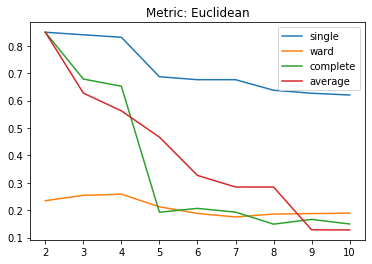
\includegraphics[width=.49\textwidth]{silueuc}\hfill
		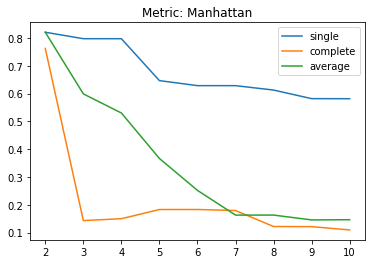
\includegraphics[width=.49\textwidth]{siluman.png}\hfill
		\caption{Silhouettes for all algorithms and all metrics on data frame 2}
		\label{fig:silu}
	\end{figure}
	From those plot, we notice a tendency for the silhouette to drop when the number of cluster passes from 4 to 5. We then decide to perform clustering with 4 clusters.
	Given that, we visually inspected the results and found that the only ones with interesting clusters are:
	\begin{itemize}
		\item Euclidean metric and ward linkage
		\item Manhattan metric and complete linkage
	\end{itemize}
	The visual result of those clustering is shown in figure \ref{fig:hier}, while their respective dendrograms are shown in figure \ref{fig:dend}. All the other clustering attempts produced highly imbalanced cluster (one main cluster and some single digit size clusters).
	\begin{figure}[H]
		\centering
		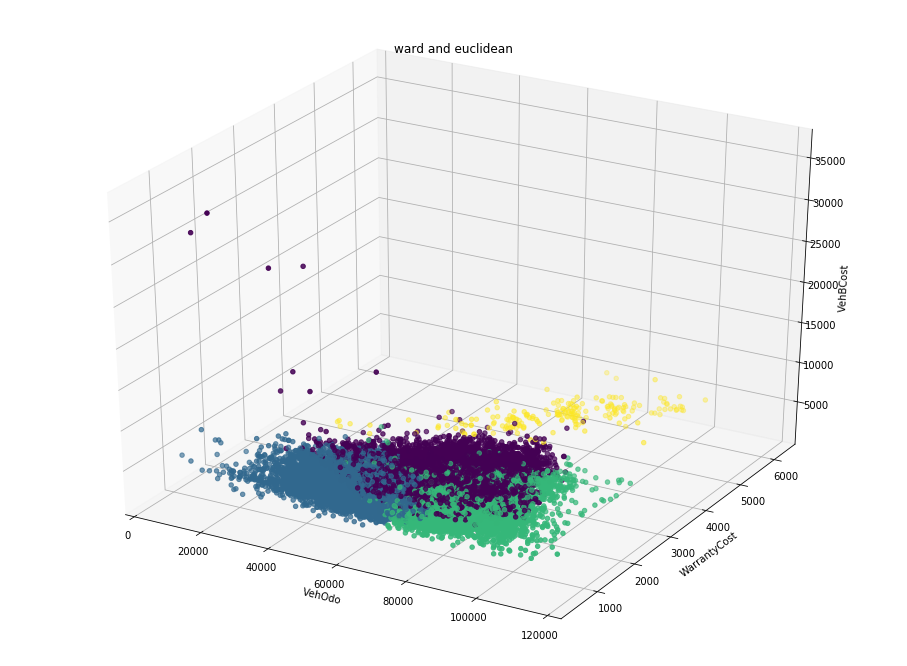
\includegraphics[width=.49\textwidth]{wardeucl}\hfill
		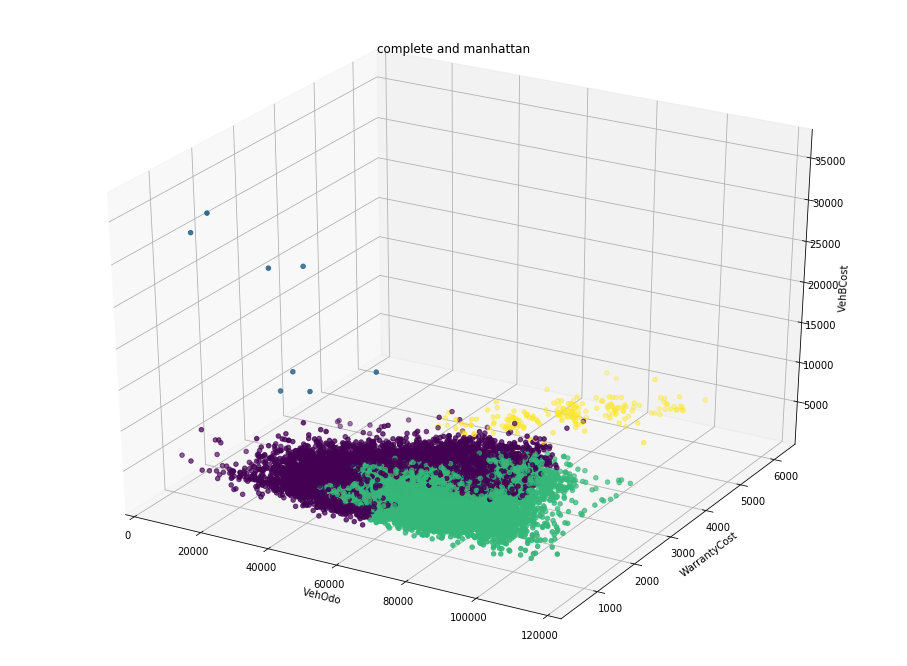
\includegraphics[width=.49\textwidth]{complman}\hfill
		\caption{Hierarchical clustering results, number of clusters is 4}
		\label{fig:hier}
	\end{figure}
	\begin{figure}[H]
		\centering
		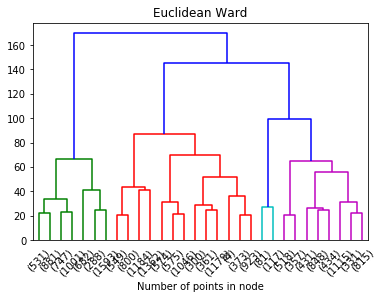
\includegraphics[width=.49\textwidth]{dendeuc}\hfill
		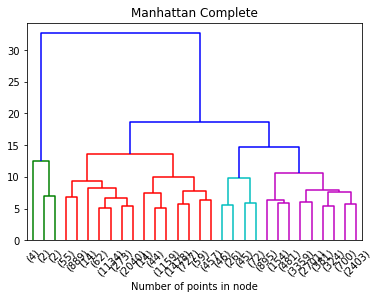
\includegraphics[width=.49\textwidth]{dendman}\hfill
		\caption{Dendrograms plotted with \emph{lastp} truncate mode}
		\label{fig:dend}
	\end{figure}
	
	
	\subsubsection{Best clustering approach and comparison of the clustering obtained}
	In conclusion, the best clustering results were found in the circumstances shown in section \ref{sec:hier}. The results, semantically speaking, highly resemble the ones found using KMeans. Both results find a cluster in the high warranty cost cars (displayed in both figure \ref{fig:hier} and in figure \ref{fig:centroid} for KMeans, where the highlighted cluster is displayed in yellow).\\
	The main difference is in the way that points in the "big cloud" are assigned a cluster. The reasoning, anyway, is really similar to the one made in section \ref{sec:clusterdescr} regarding KMeans, so we refer to that one.
	
	
	
	
	\section{Classification}
	\label{sec:classification}
	In the following section, we describe the methodologies and the algorithms used during the classification. The main goal of this task was to predict the variable called \textit{"IsBadBuy"}, that indicates whether a car has been a good business or not.
	
	\subsection{Hyper-parameters Optimization}
	To discover the best way to predict the required variable, we tested a lot of models by optimizing their hyper-parameters. Those act as knobs to fine-tune the model, so to provide the best result, we need to find out the optimal value of these parameters, or in other words, a trade-off between true/false positives and true/false negatives. Since each algorithm has its peculiarity, for each classificator, we created different groups of parameters to experiment. Table \ref{tab:hyper} shows the setup of our analyses.
	
	
	\begin{table}[H]
		\begin{center}
			\begin{tabular}{ c | c }
				\hline
				\textbf{Algorithm} & \textbf{Hyper-parameters}\\
				\hline
				\rowcolor{Gray}
				Random Forest & \textit{n\_estimators}: 25, 50, 100, 200, 500, 1000 \\
				\hline
				Decision Tree & \specialcell{
					\textit{criterion} : 'gini', 'entropy'\\
					\textit{max\_depth} : 2, 5, 10, 15, None\\
					\textit{min\_samples\_split} : 2, 5, 10, 20}\\
				\hline
				\rowcolor{Gray}
				AdaBoost & \specialcell{
					\textit{n\_estimators} : 5, 10, 25, 50, 100 \\
					\textit{learning\_rate} : 0.1, 0.25, 0.5, 0.75, 1} \\
				\hline
				KNN & \specialcell{
					\textit{n\_neighbors} : 1, 4, 7, 10, 13, 16, 19, 22, 25, 28 \\
					\textit{weights} : 'uniform', 'distance' } \\
				\hline
			\end{tabular}
		\end{center}
		\caption{Setup environment of the tested hyper-parameters}
		\label{tab:hyper}
	\end{table}
	
	
	\subsubsection{Methodology}
	The first step was to isolate the test set ("test.csv") because this will be used as ground truth to verify the performance of the created models. Then, we cross-validate each model by using as input data, the given training set ("training.csv"). To reflect the percentage of the initial datasets, we decided to split the data in 60-40 (respectively training and validation). For each algorithm of classification, and for each tuple of parameters, we performed 5 Cross-Validation and we averaged the results to circumvent overfitting/underfitting. Do note that to improve the classes imbalance, undersampling and oversampling techniques have been applied.
	
	\subsection{Results}
	The following pictures show the performance obtained by each algorithm during the optimization. Our strategy was to focus more on optimizing Recall and F1 because our goal was to discover "bad buys". The yellow dots/squares represent our best choice of hyper-parameters. Overall the most suitable classifier for this task were decision trees and random forest.
	
	\subsubsection{Random Forest}
	
	\begin{figure}[H]
		\centering
		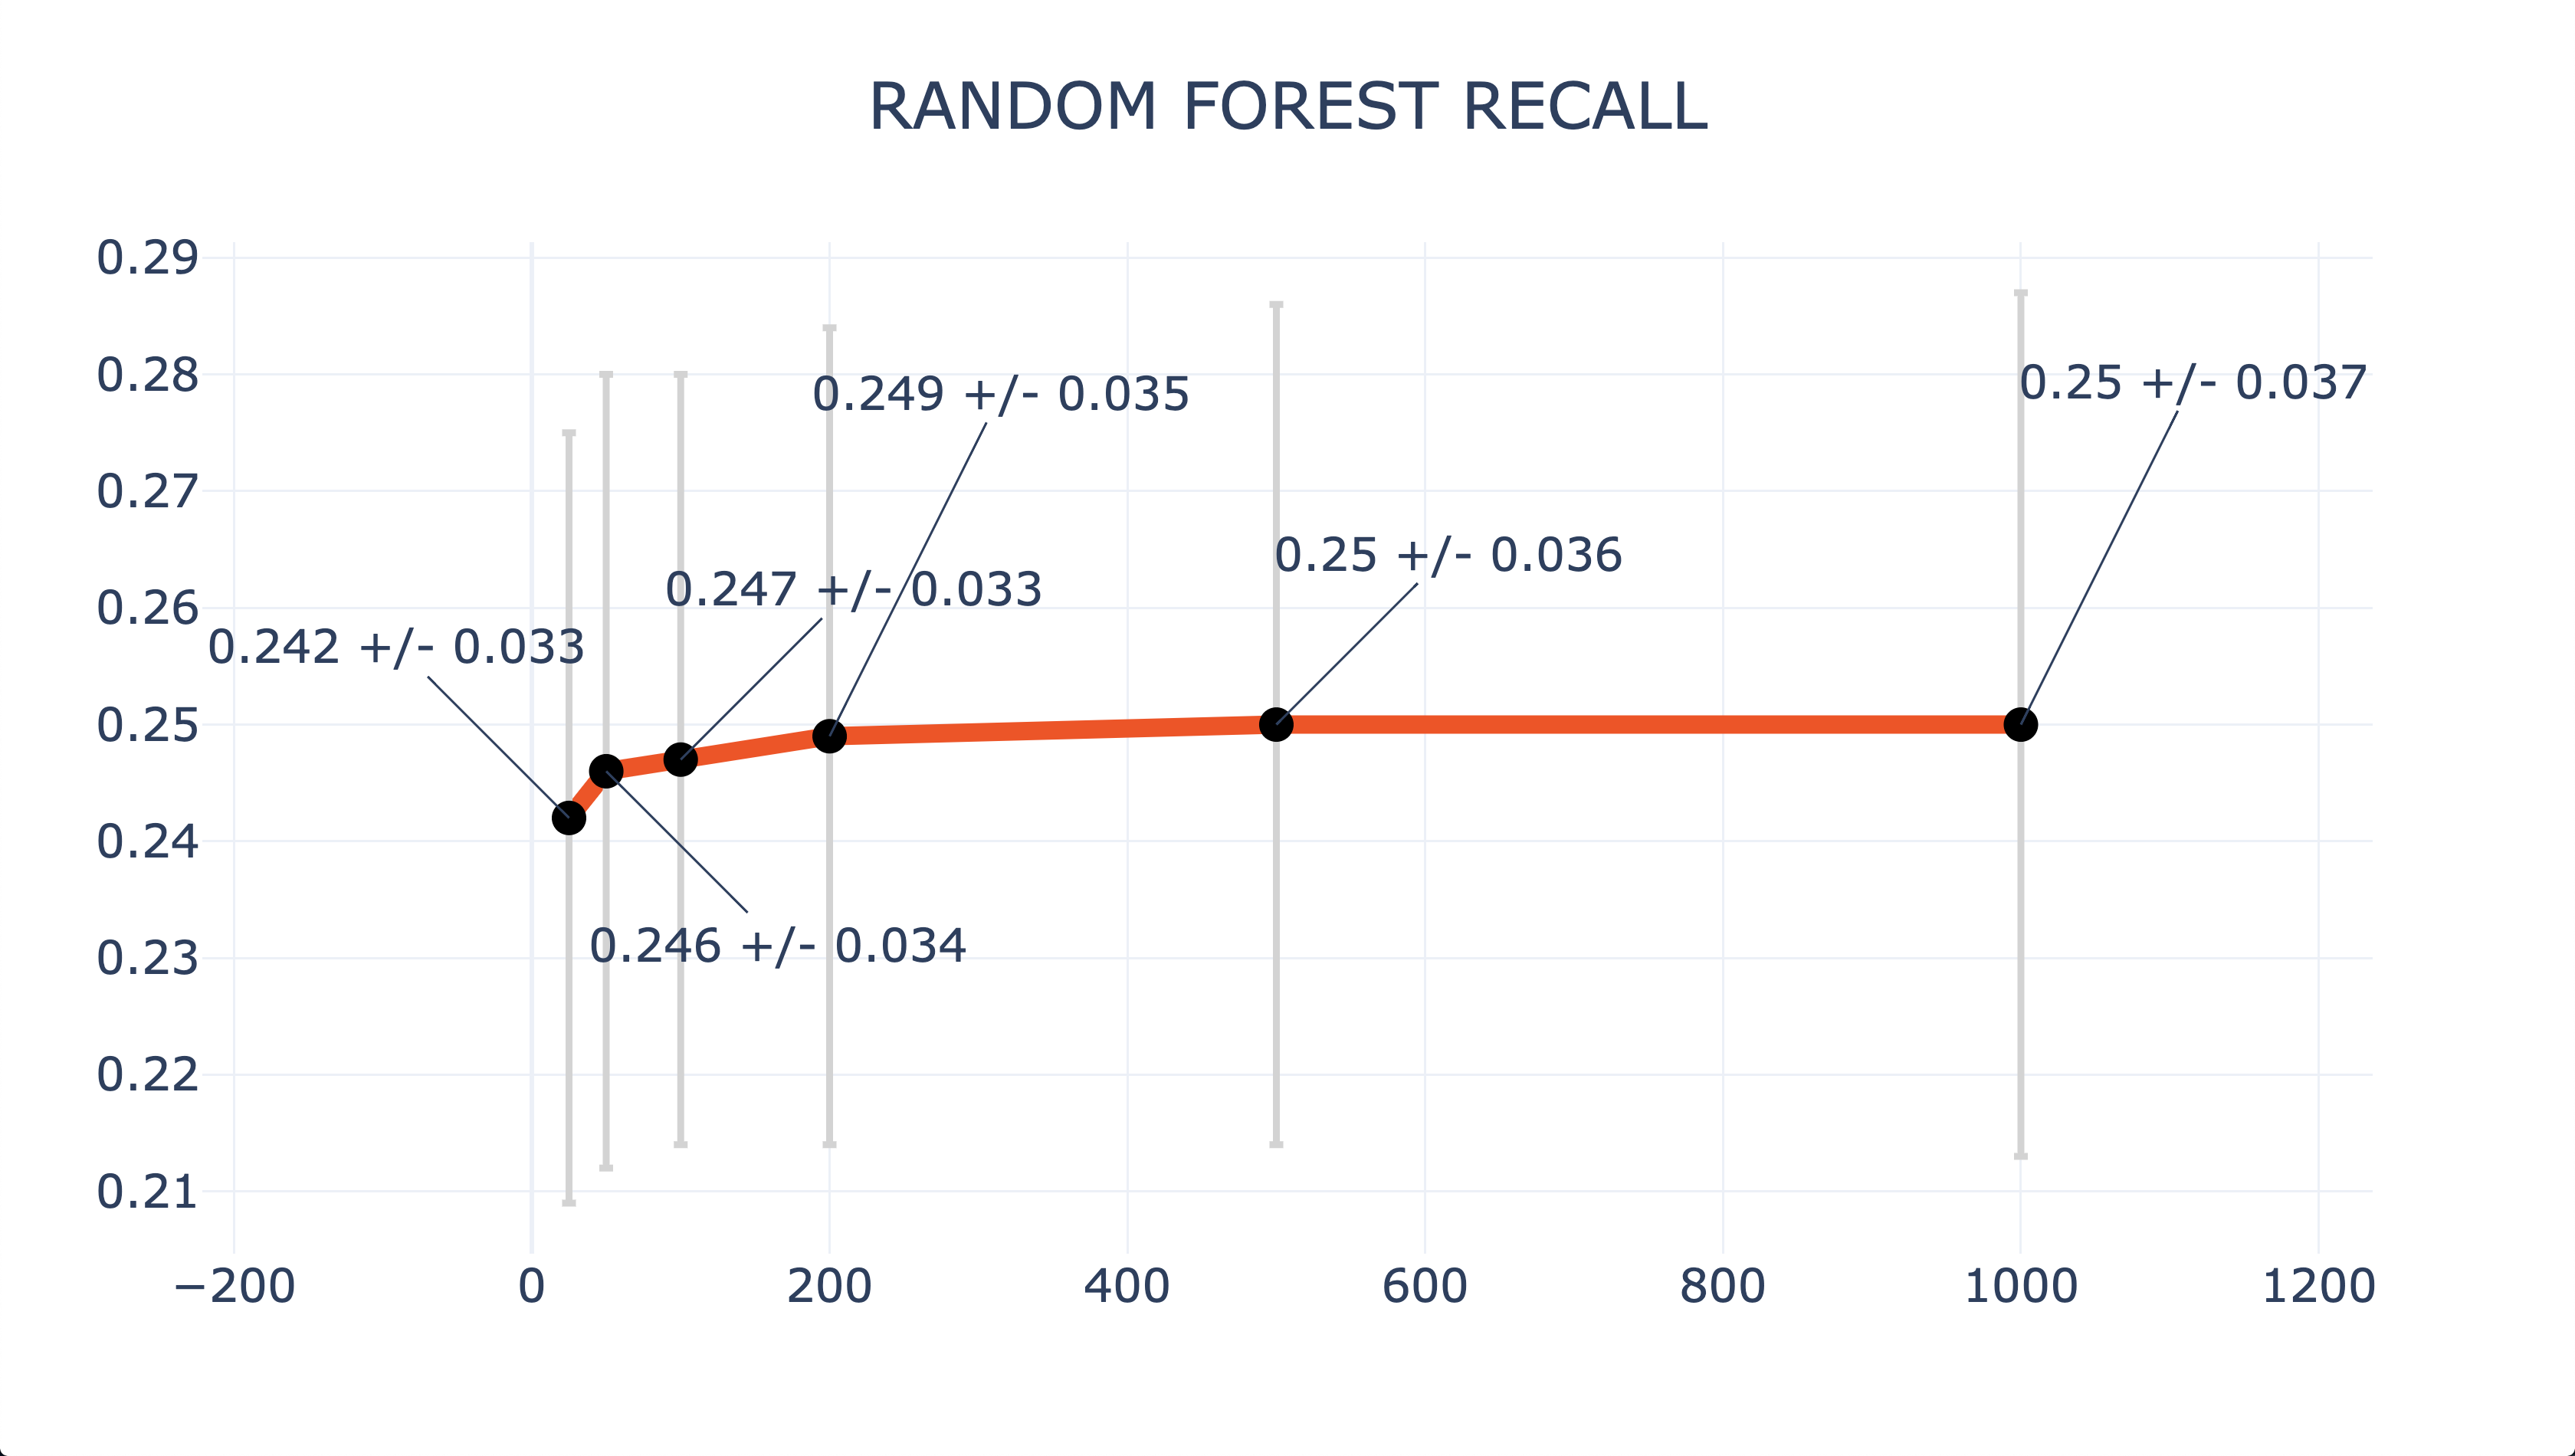
\includegraphics[width=.49\textwidth]{clf_img/RF_recall.png}
		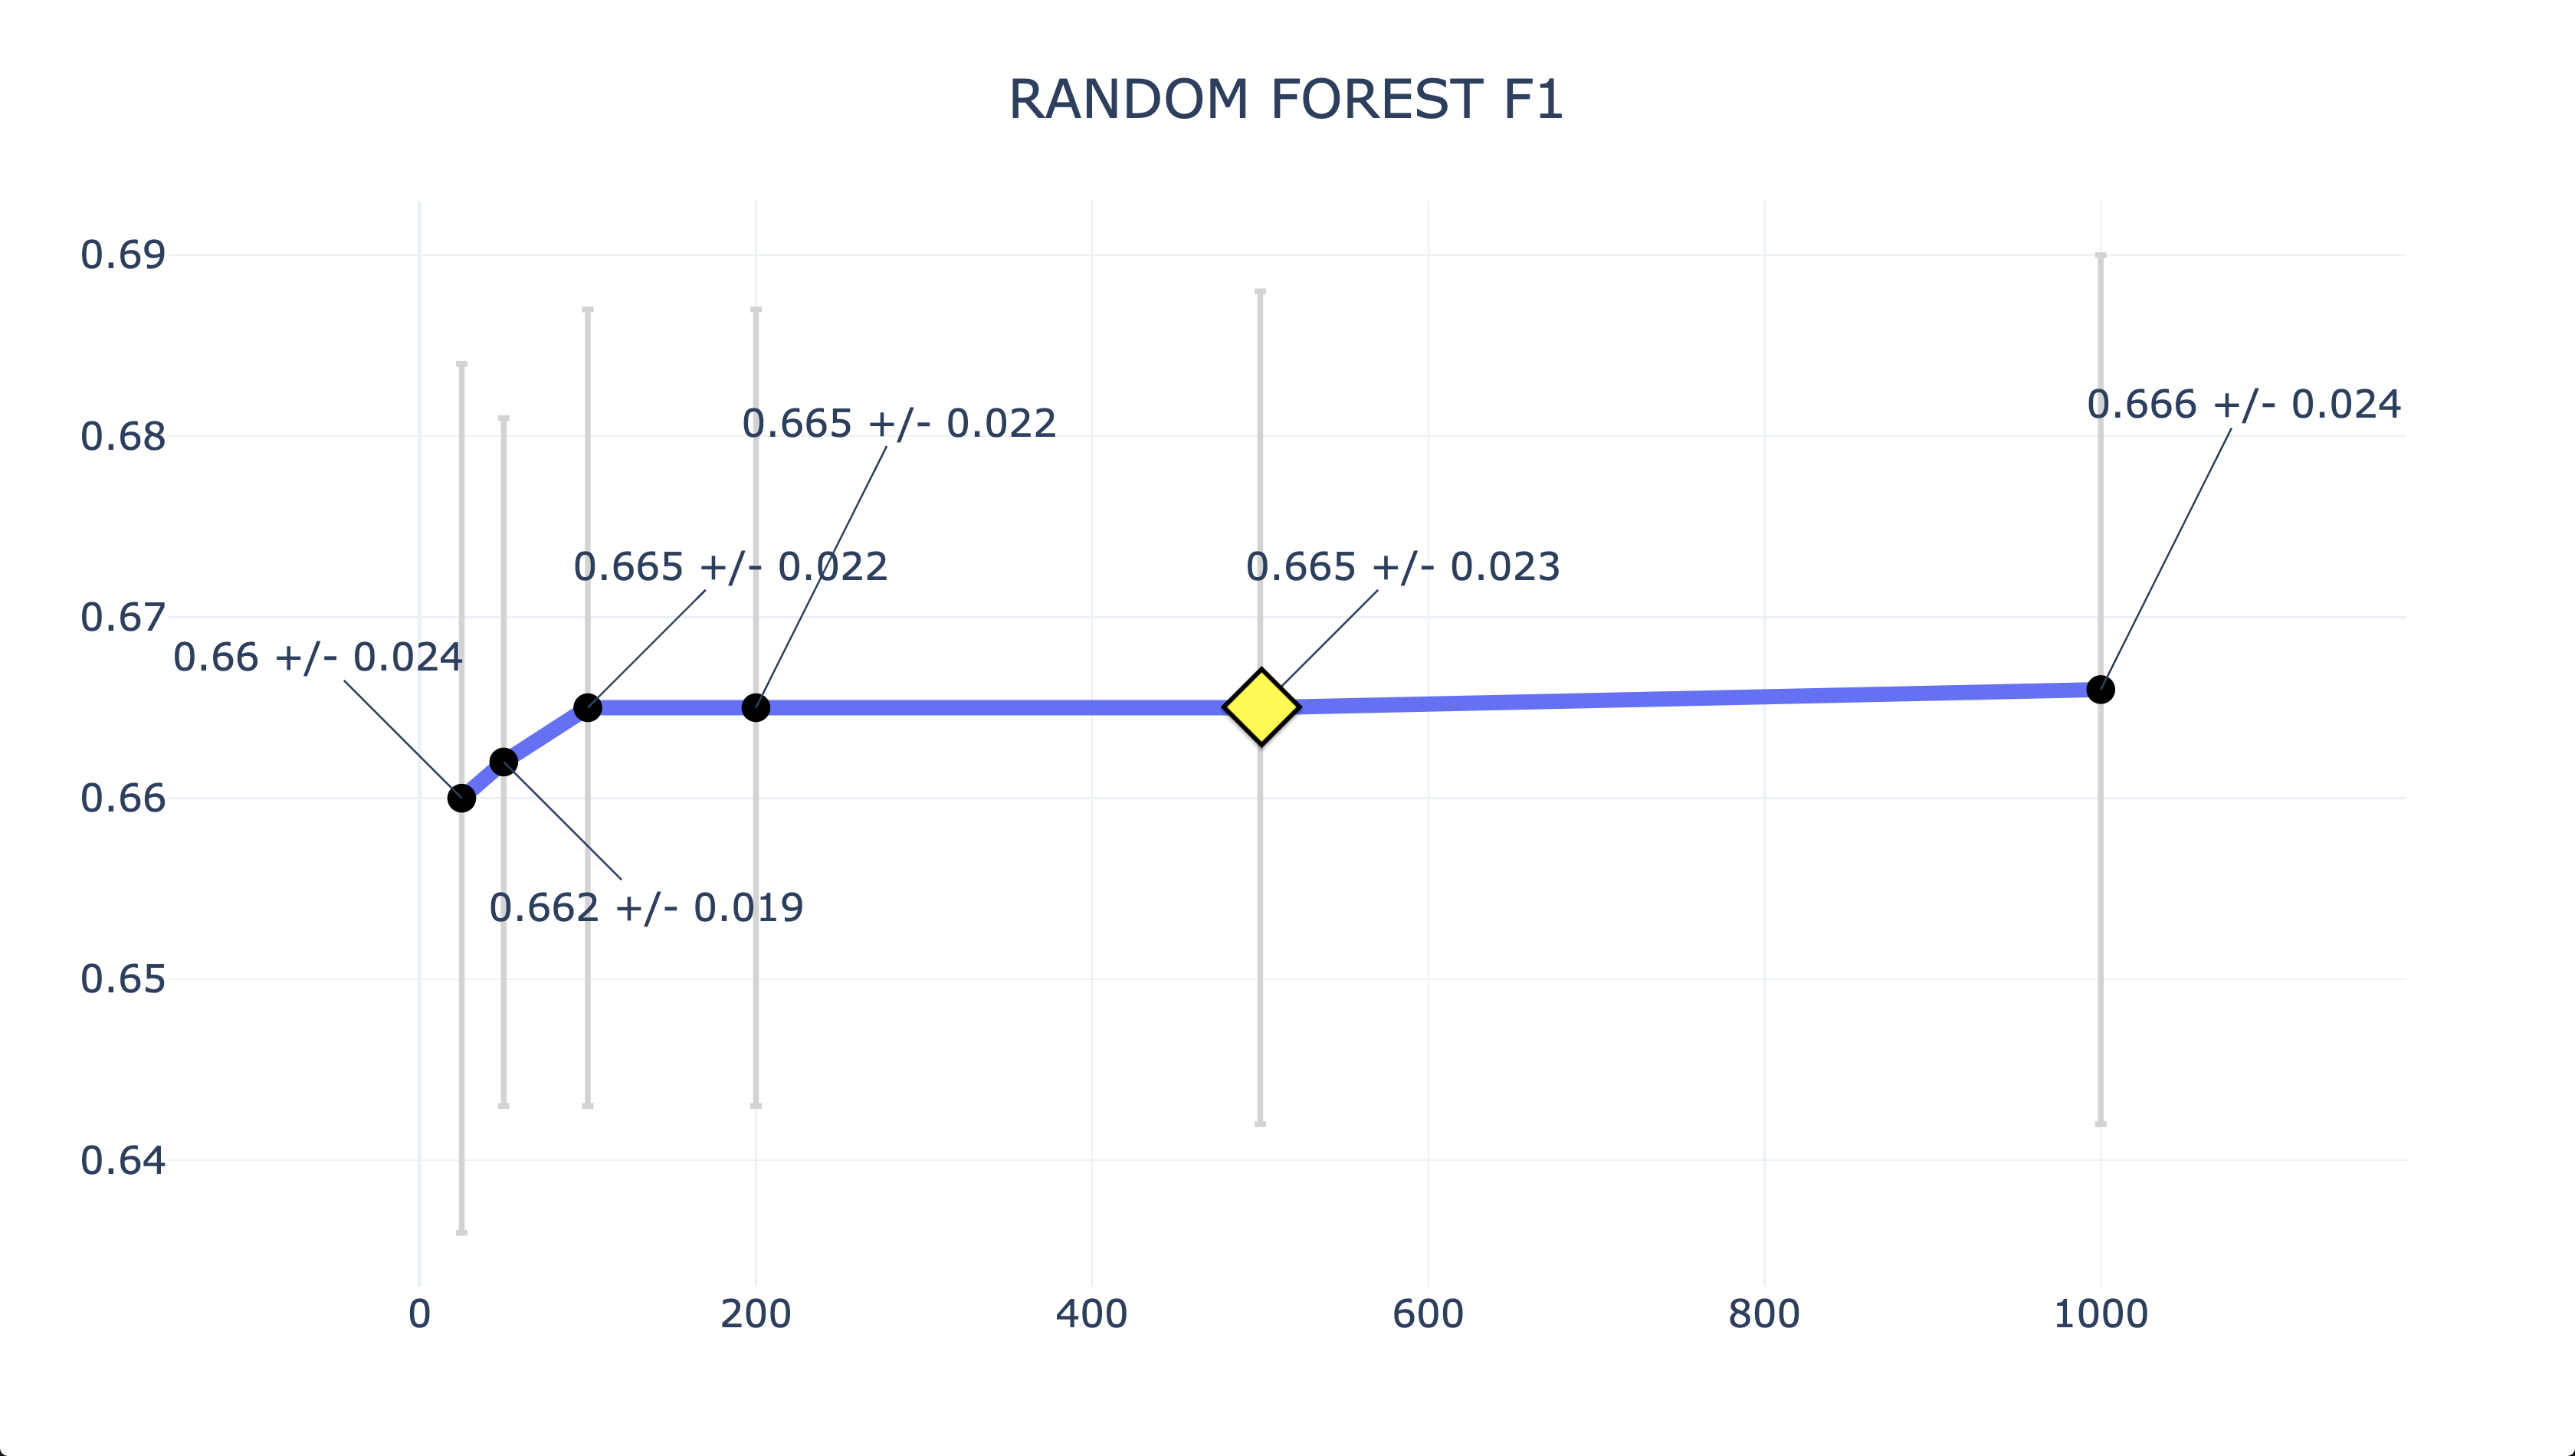
\includegraphics[width=.49\textwidth]{clf_img/RF_f1.png}
		\caption{Random Forest tuning}
		\label{fig:hyper_rf}
	\end{figure}
	
	\begin{figure}[H]
		\centering
		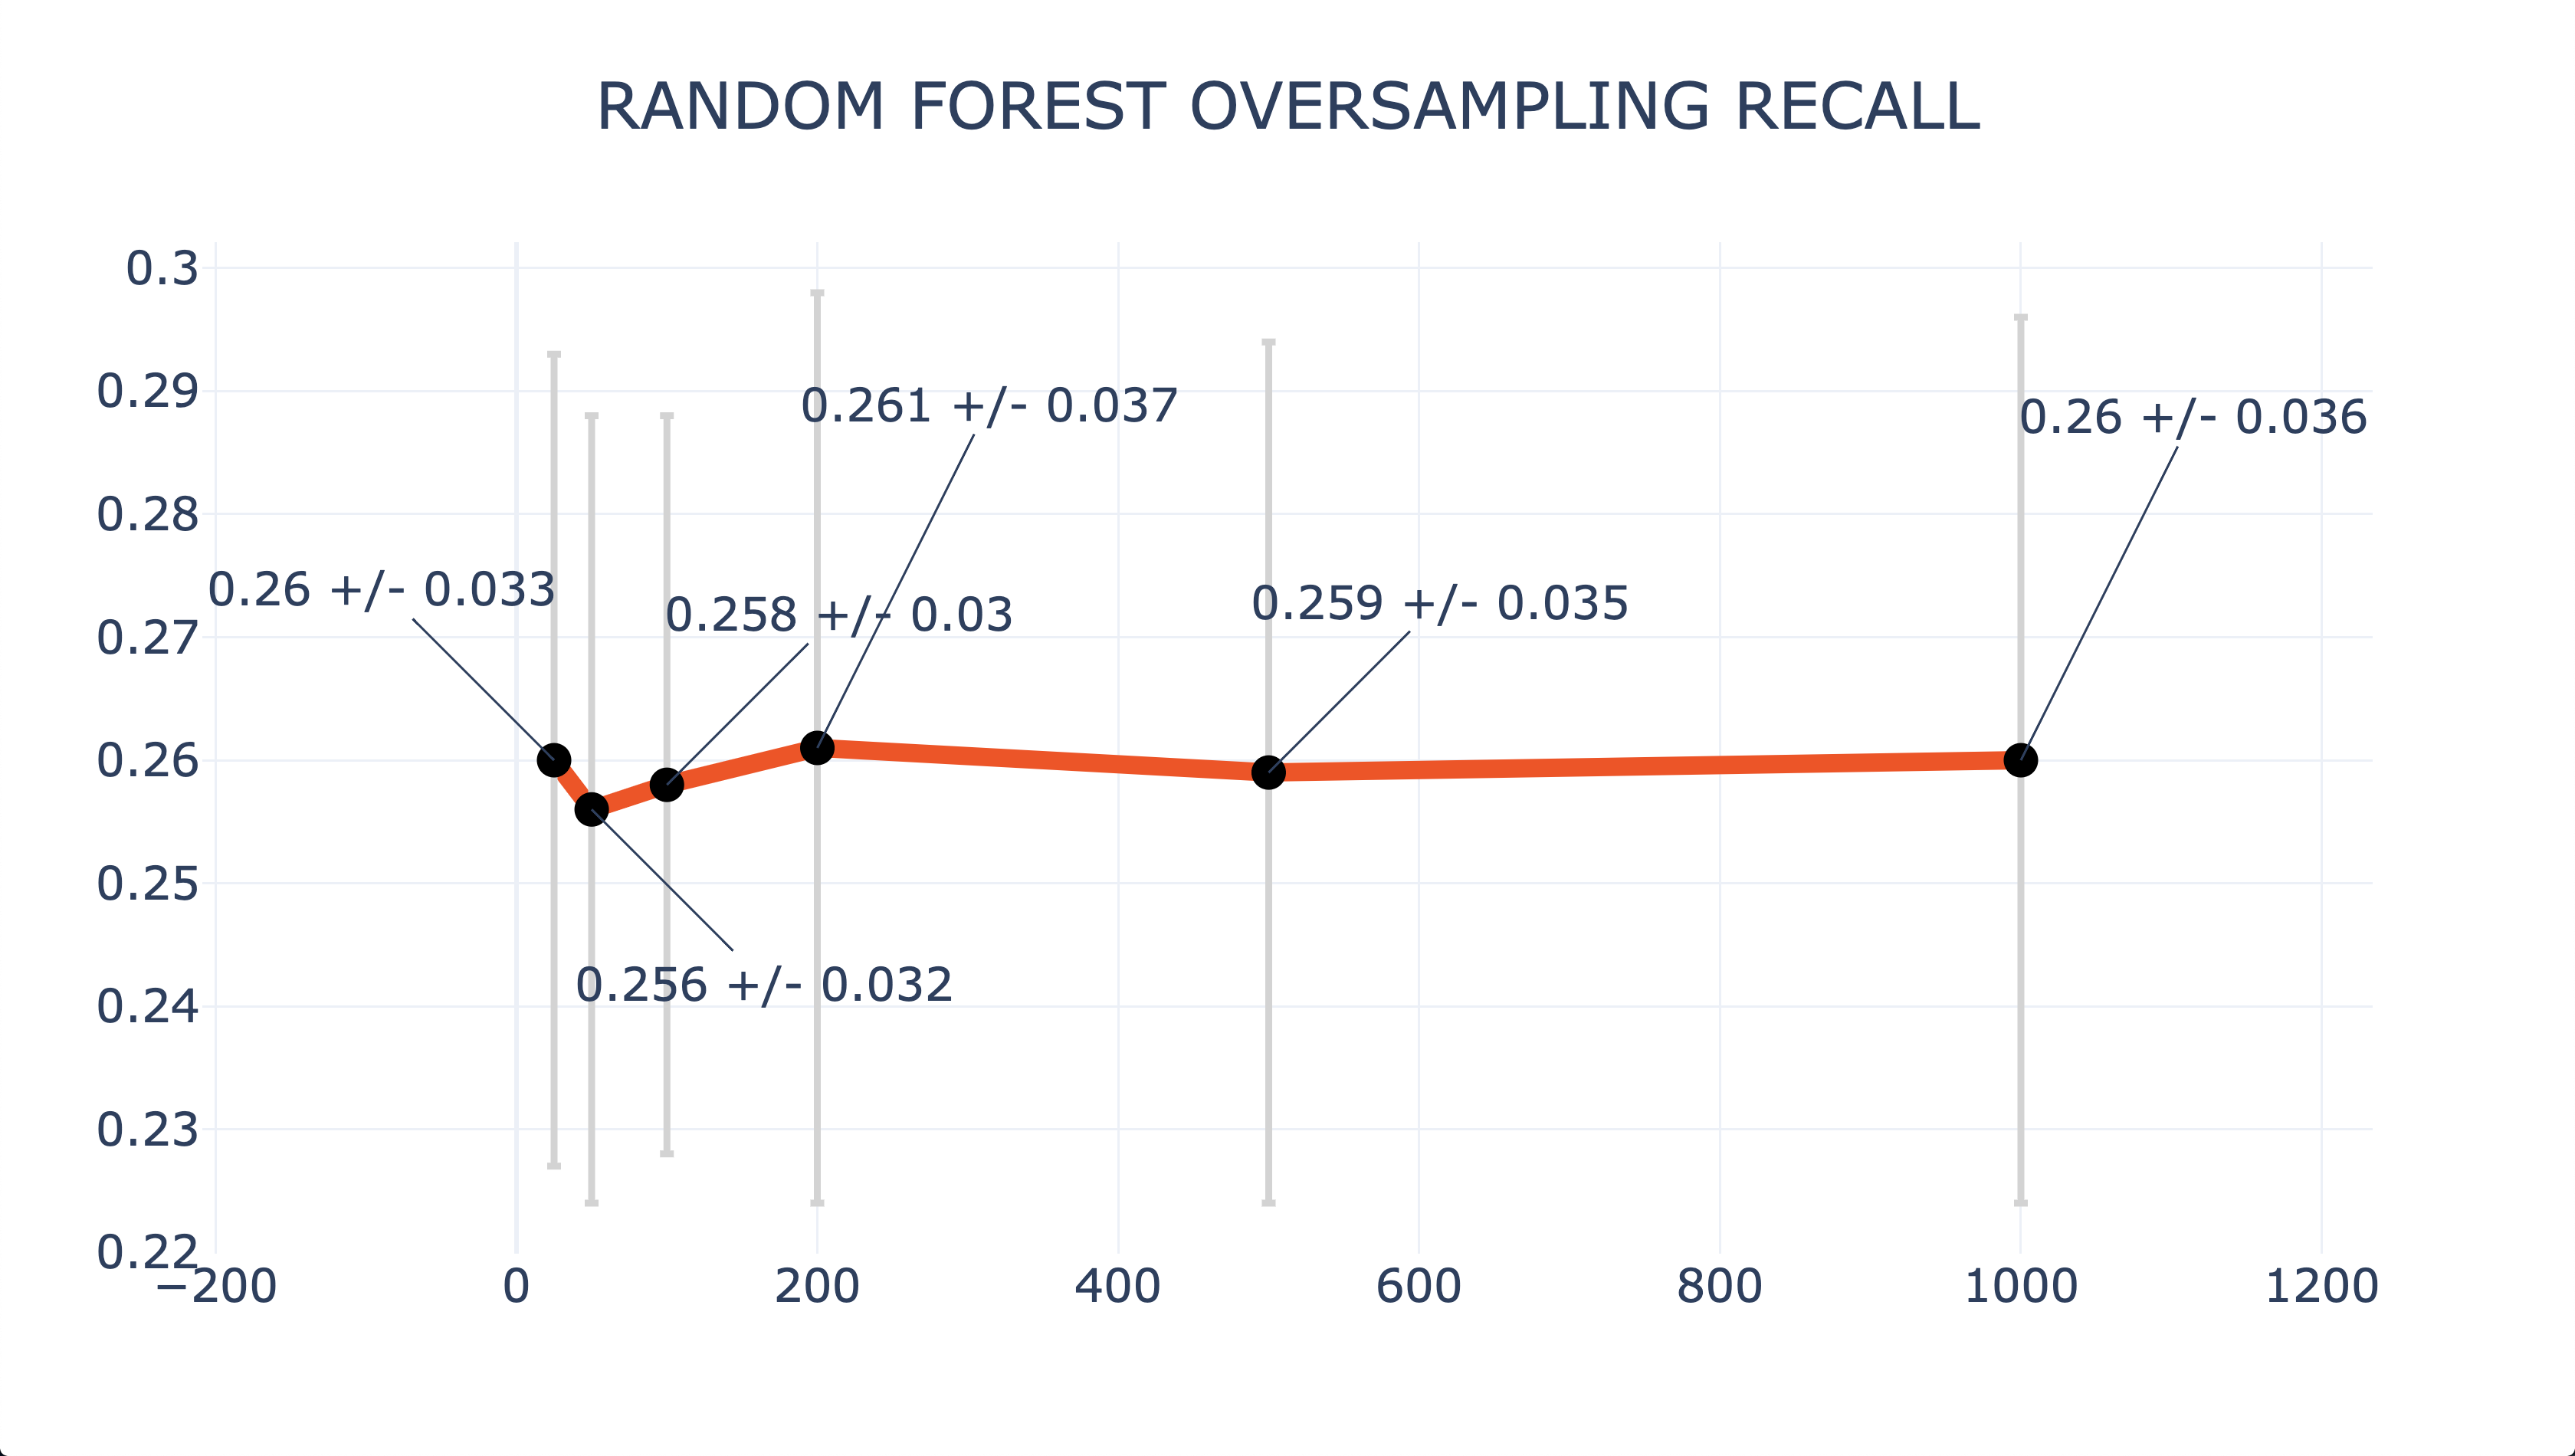
\includegraphics[width=.49\textwidth]{clf_img/RF_OS_recall.png}
		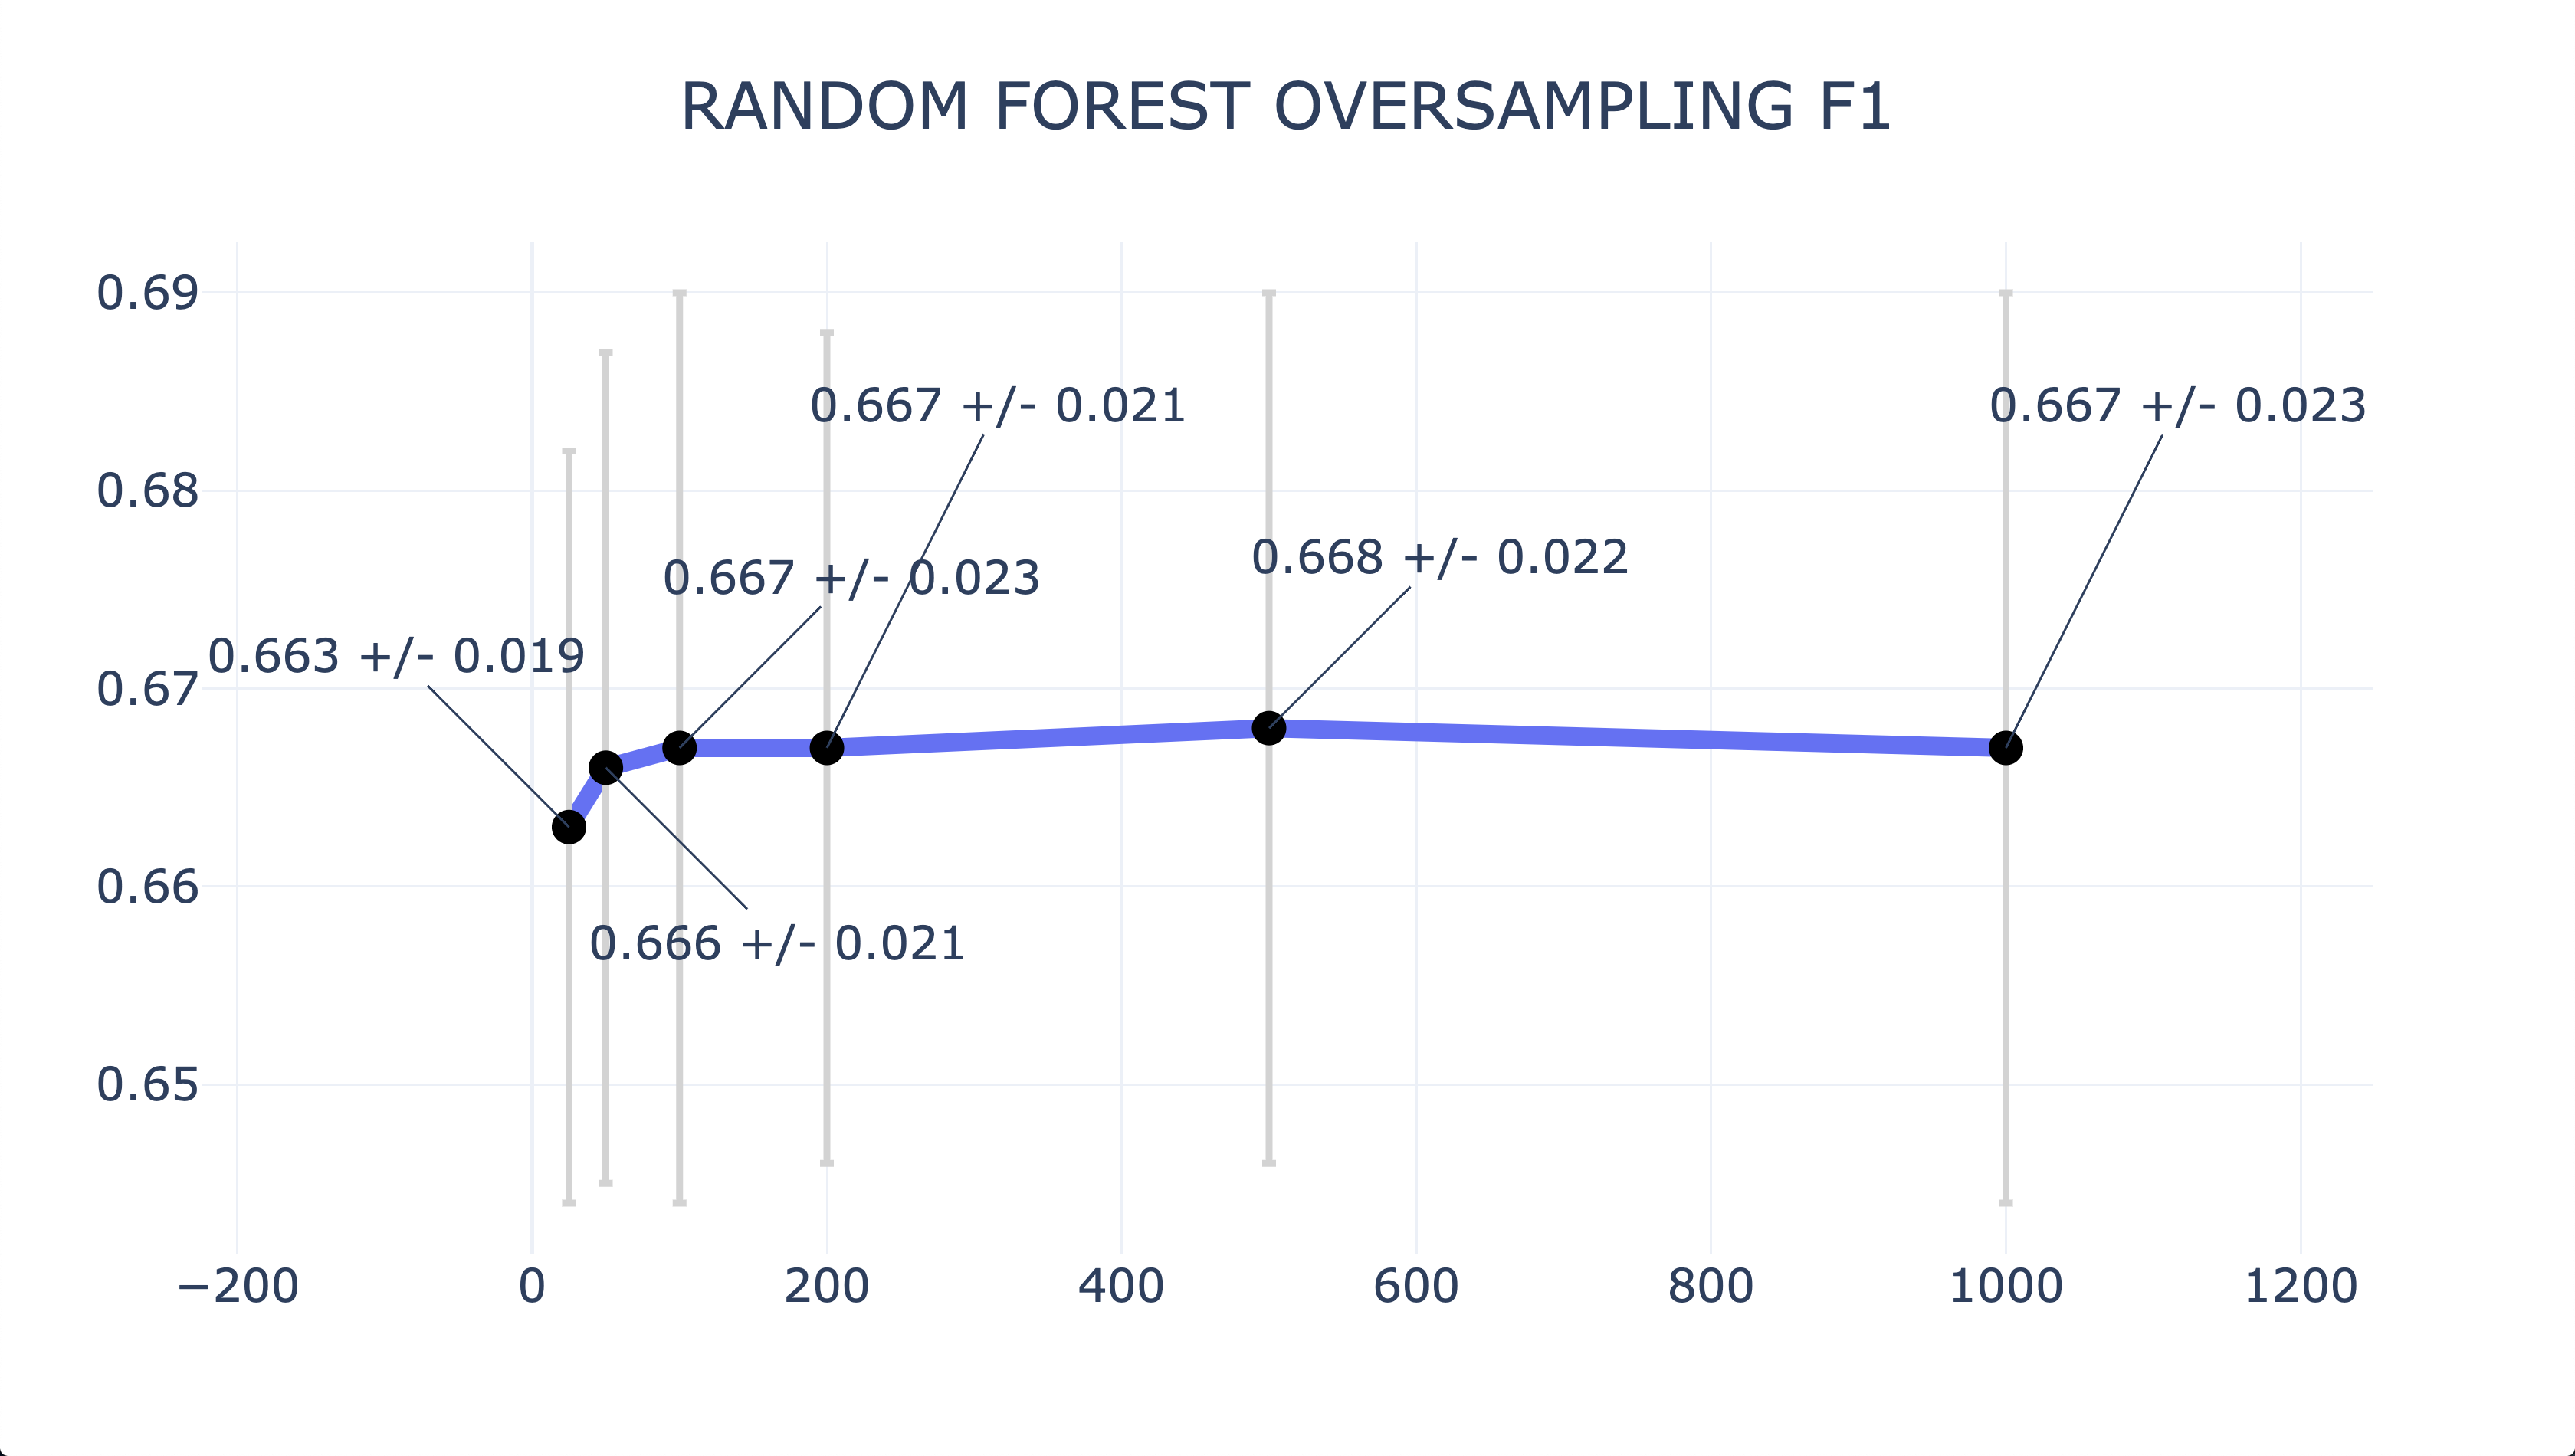
\includegraphics[width=.49\textwidth]{clf_img/RF_OS_f1.png}
		\caption{Random Forest + Oversampling tuning}
		\label{fig:hyper_rf_os}
	\end{figure}
	
	\begin{figure}[H]
		\centering
		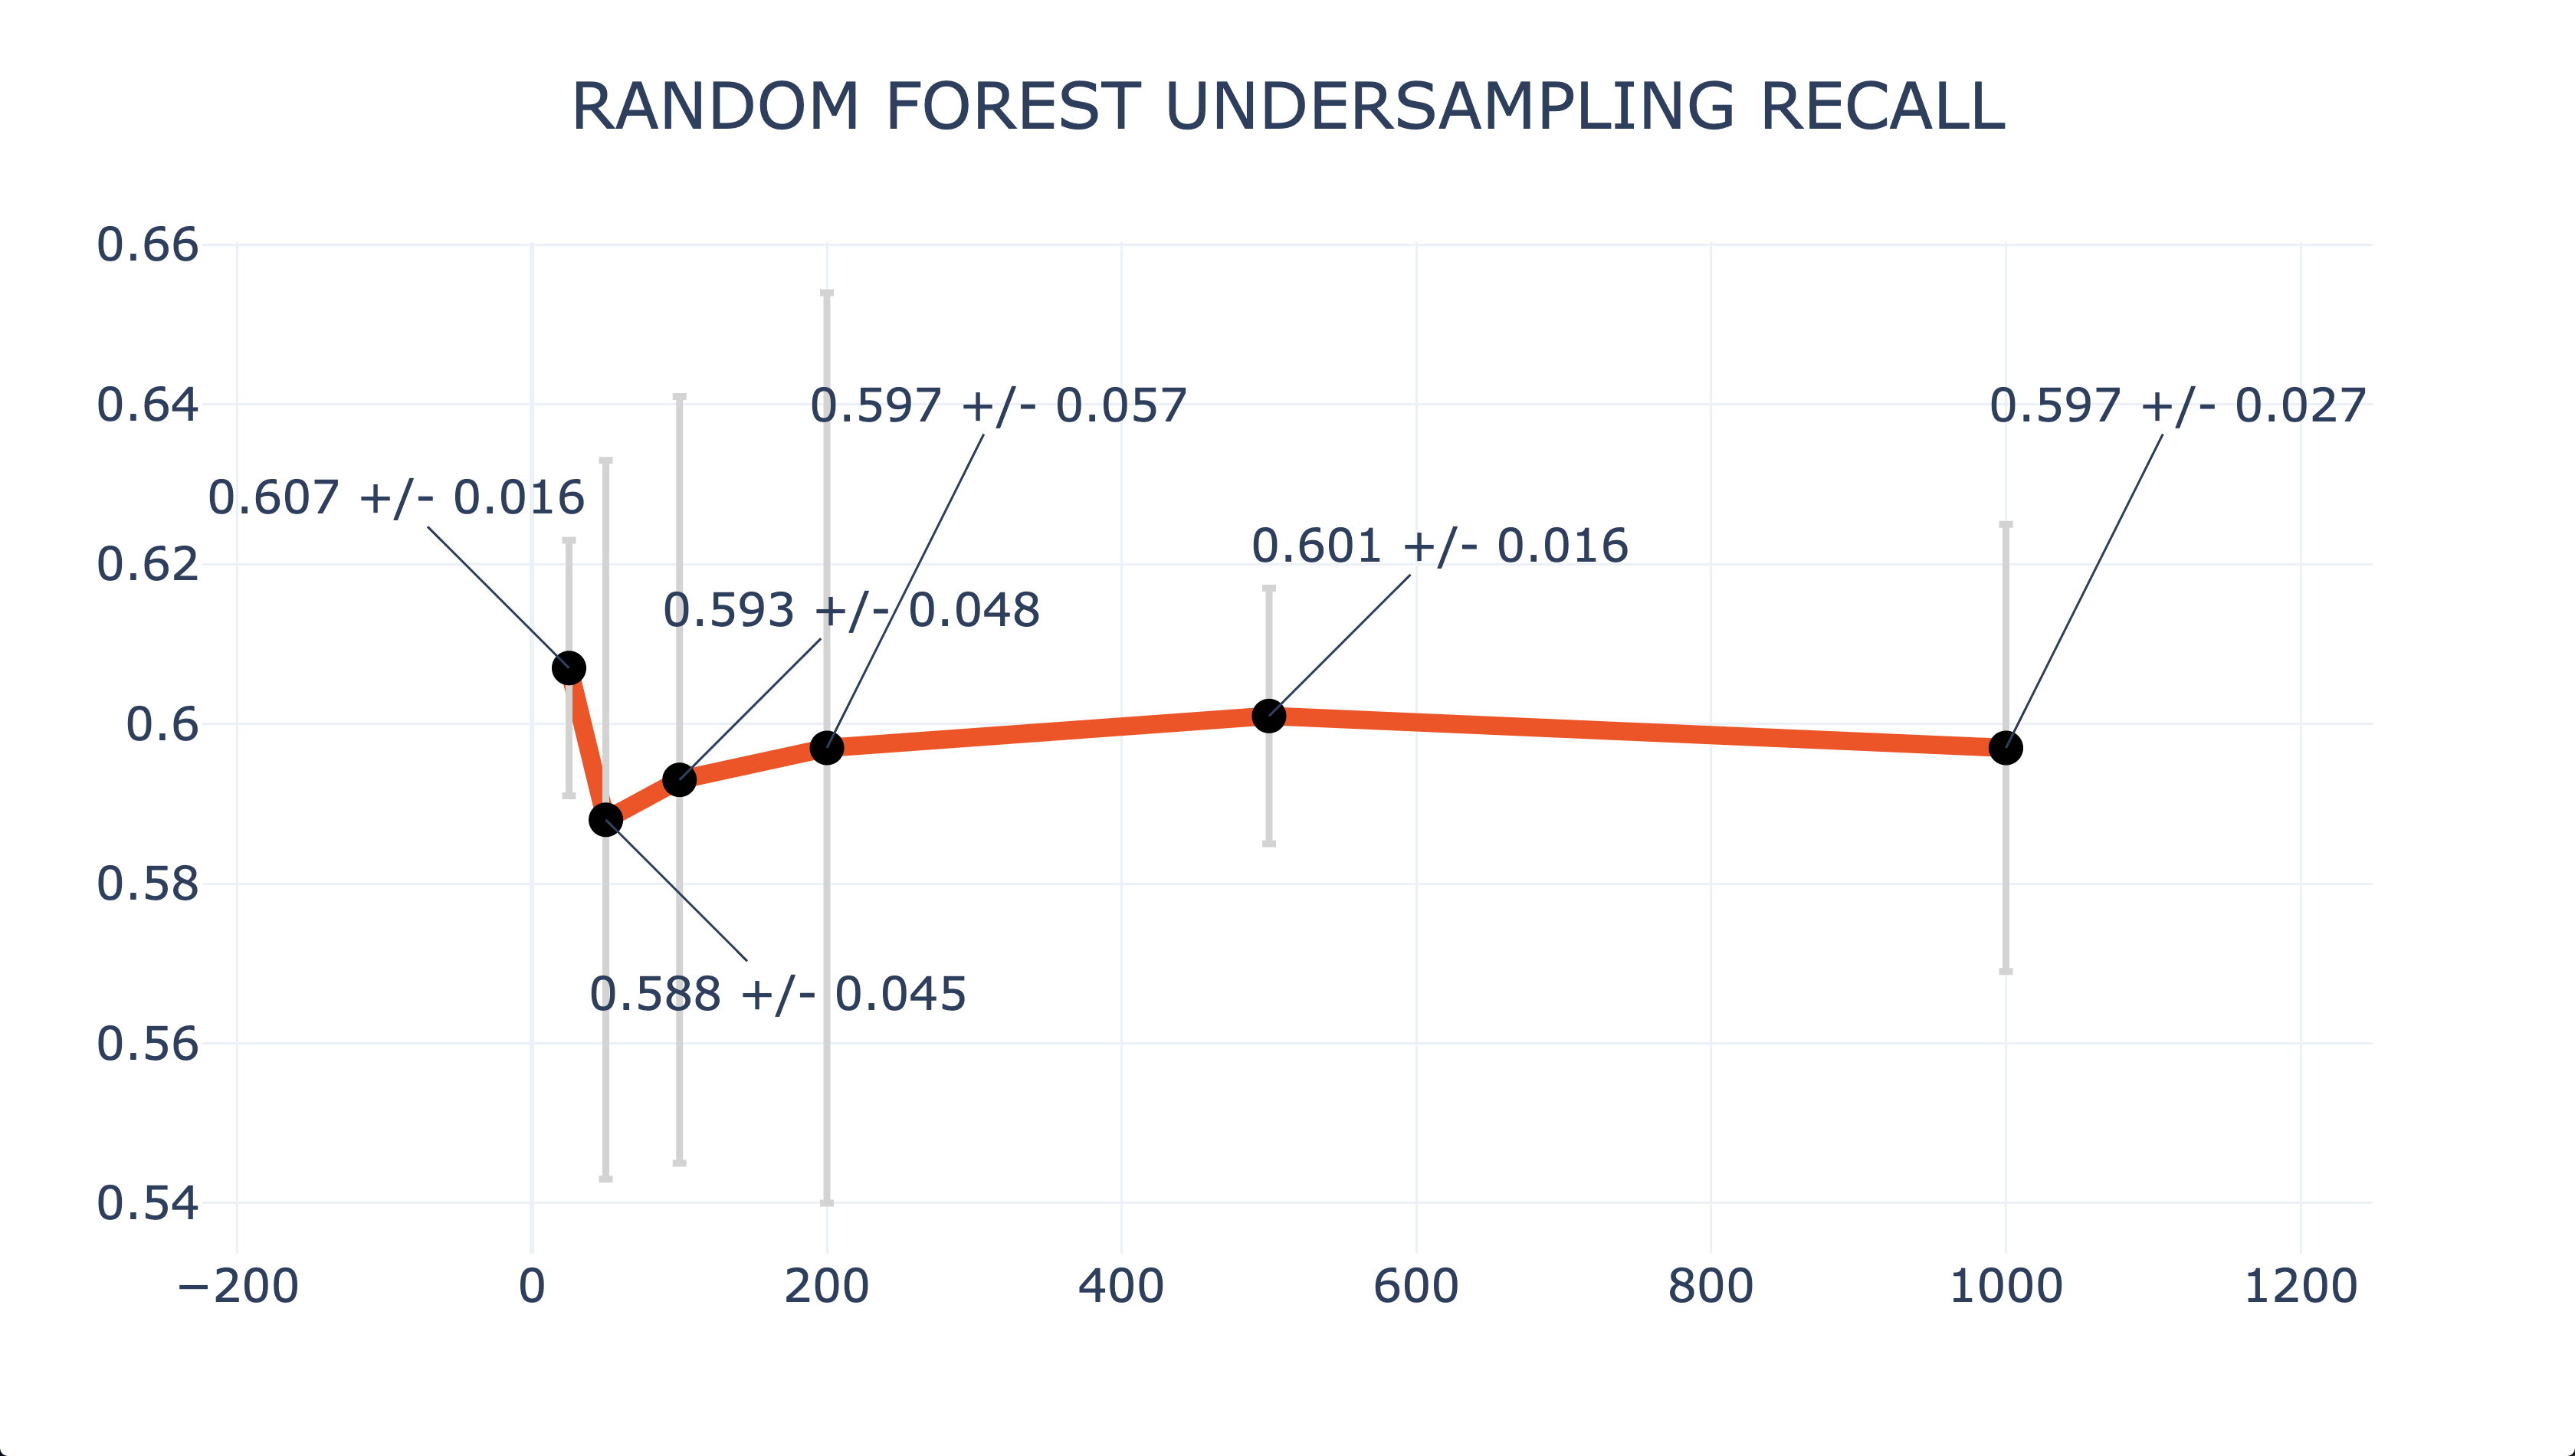
\includegraphics[width=.49\textwidth]{clf_img/RF_US_recall.png}
		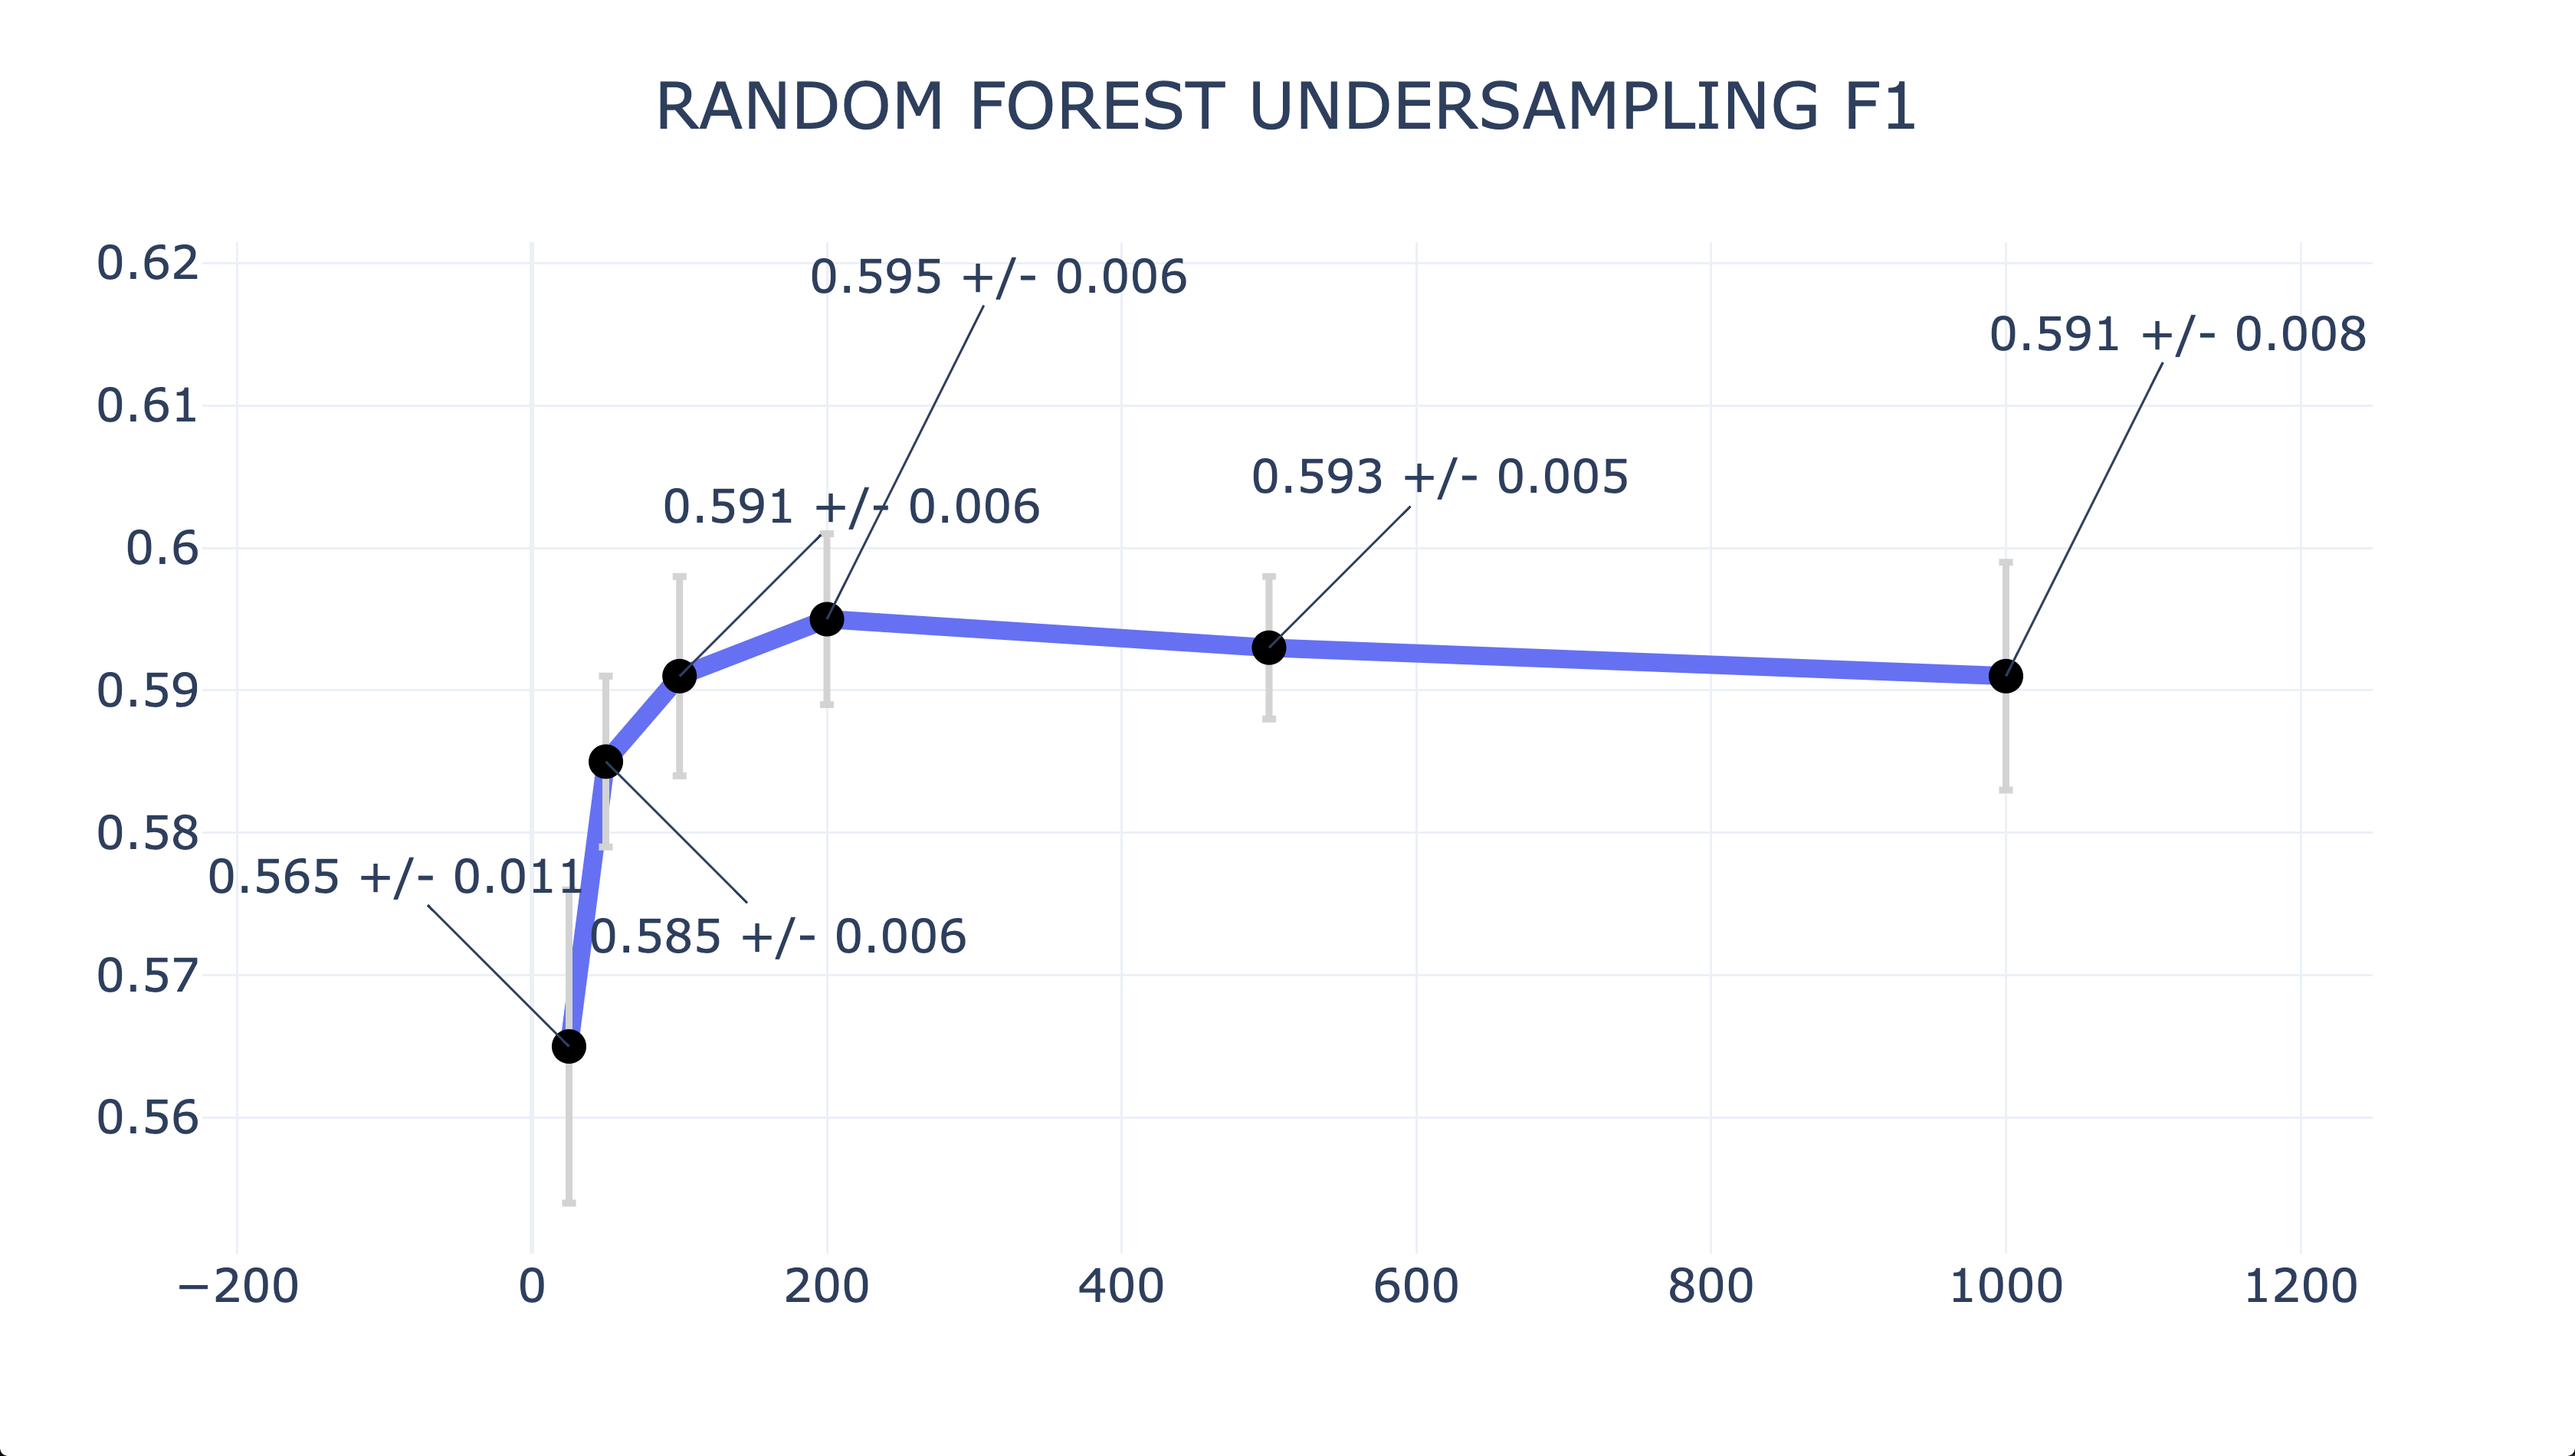
\includegraphics[width=.49\textwidth]{clf_img/RF_US_f1.png}
		\caption{Random Forest + Undersampling tuning}
		\label{fig:hyper_rf_us}
	\end{figure}
	
	
	\subsubsection{Decision Tree}
	\begin{figure}[H]
		\centering
		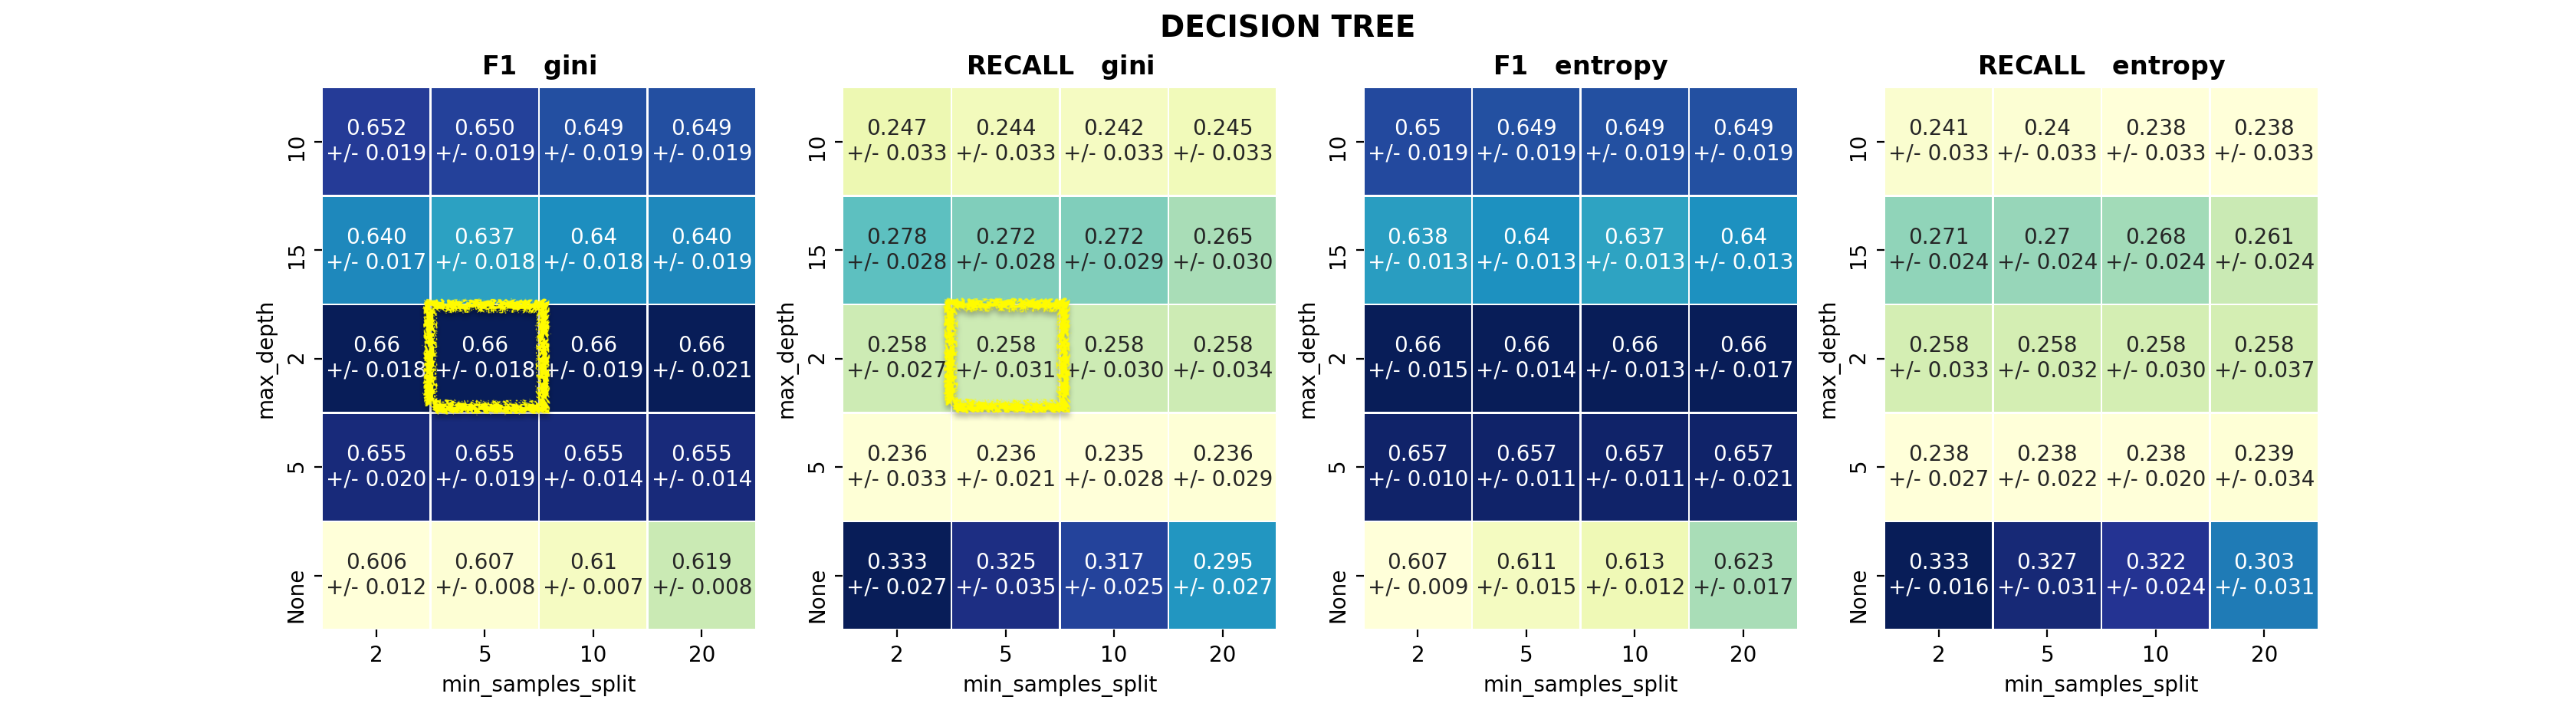
\includegraphics[width=.9\textwidth]{clf_img/DecisionTree.png}
		\caption{Decision Tree tuning}
		\label{fig:hyper_dectree}
	\end{figure}
	
	\begin{figure}[H]
		\centering
		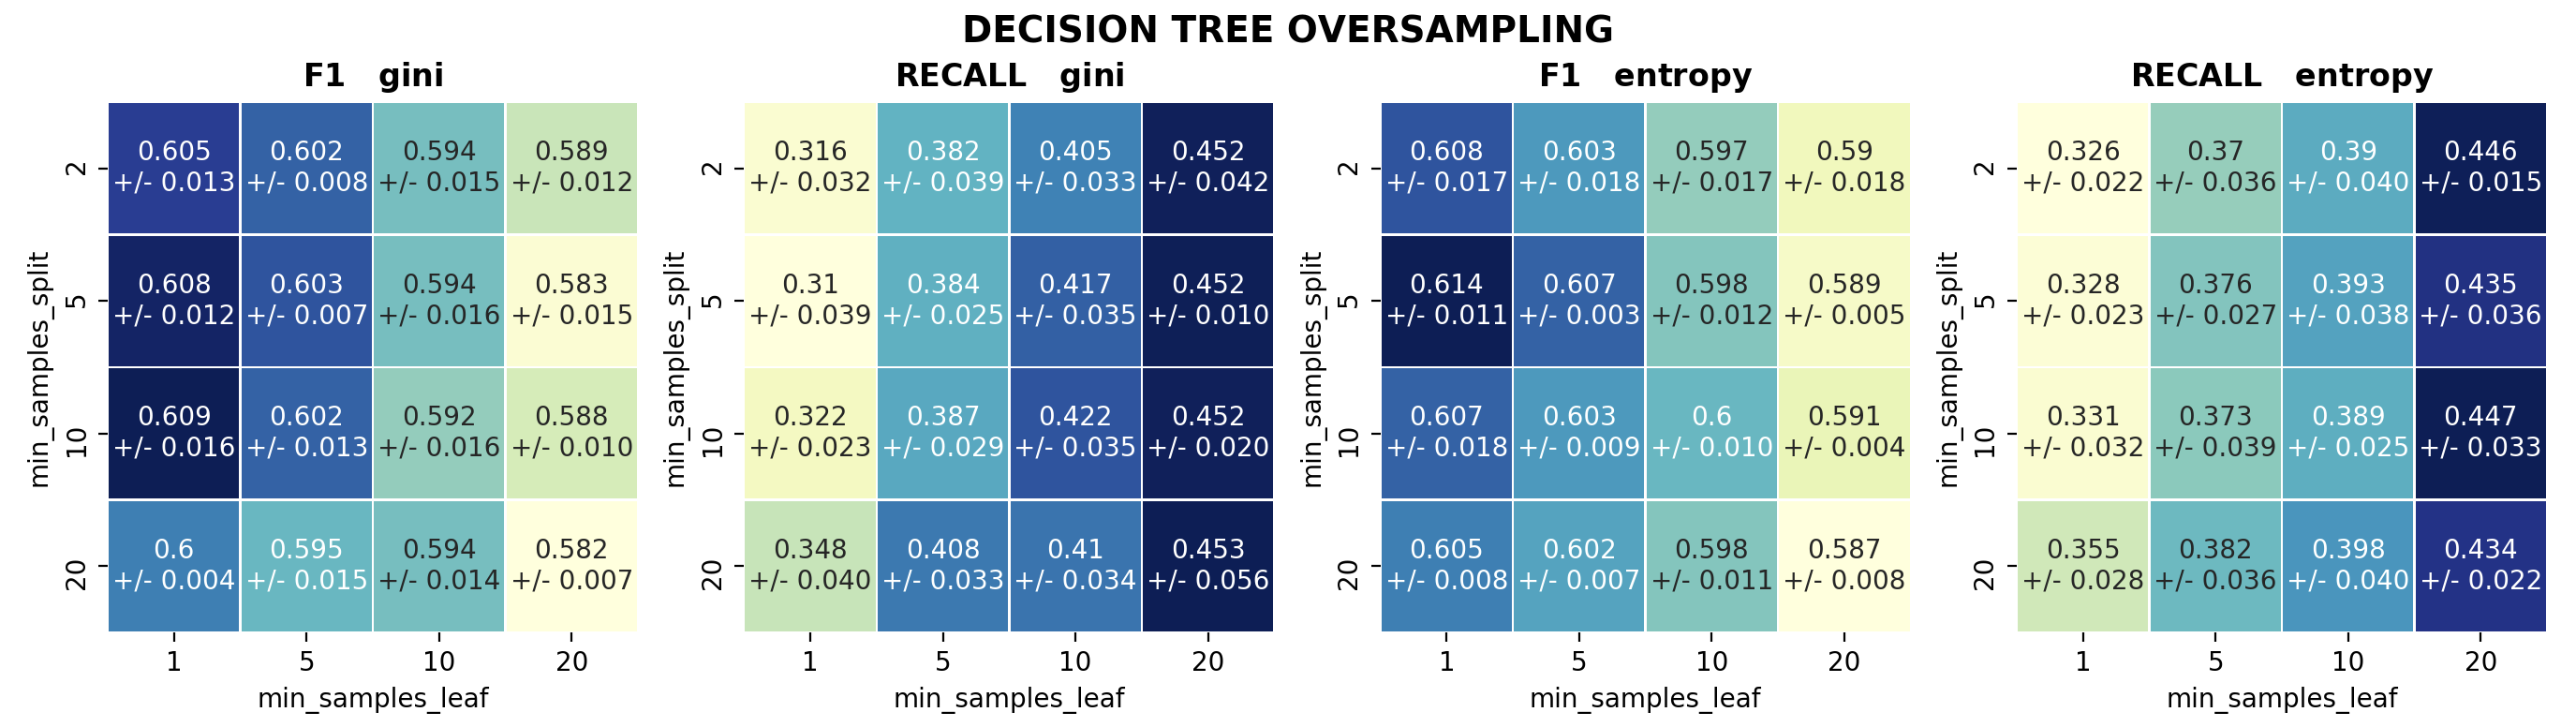
\includegraphics[width=.9\textwidth]{clf_img/DecisionTree_OS.png}
		\caption{Decision Tree + Oversampling tuning}
		\label{fig:hyper_dectreeOS}
	\end{figure}
	
	\begin{figure}[H]
		\centering
		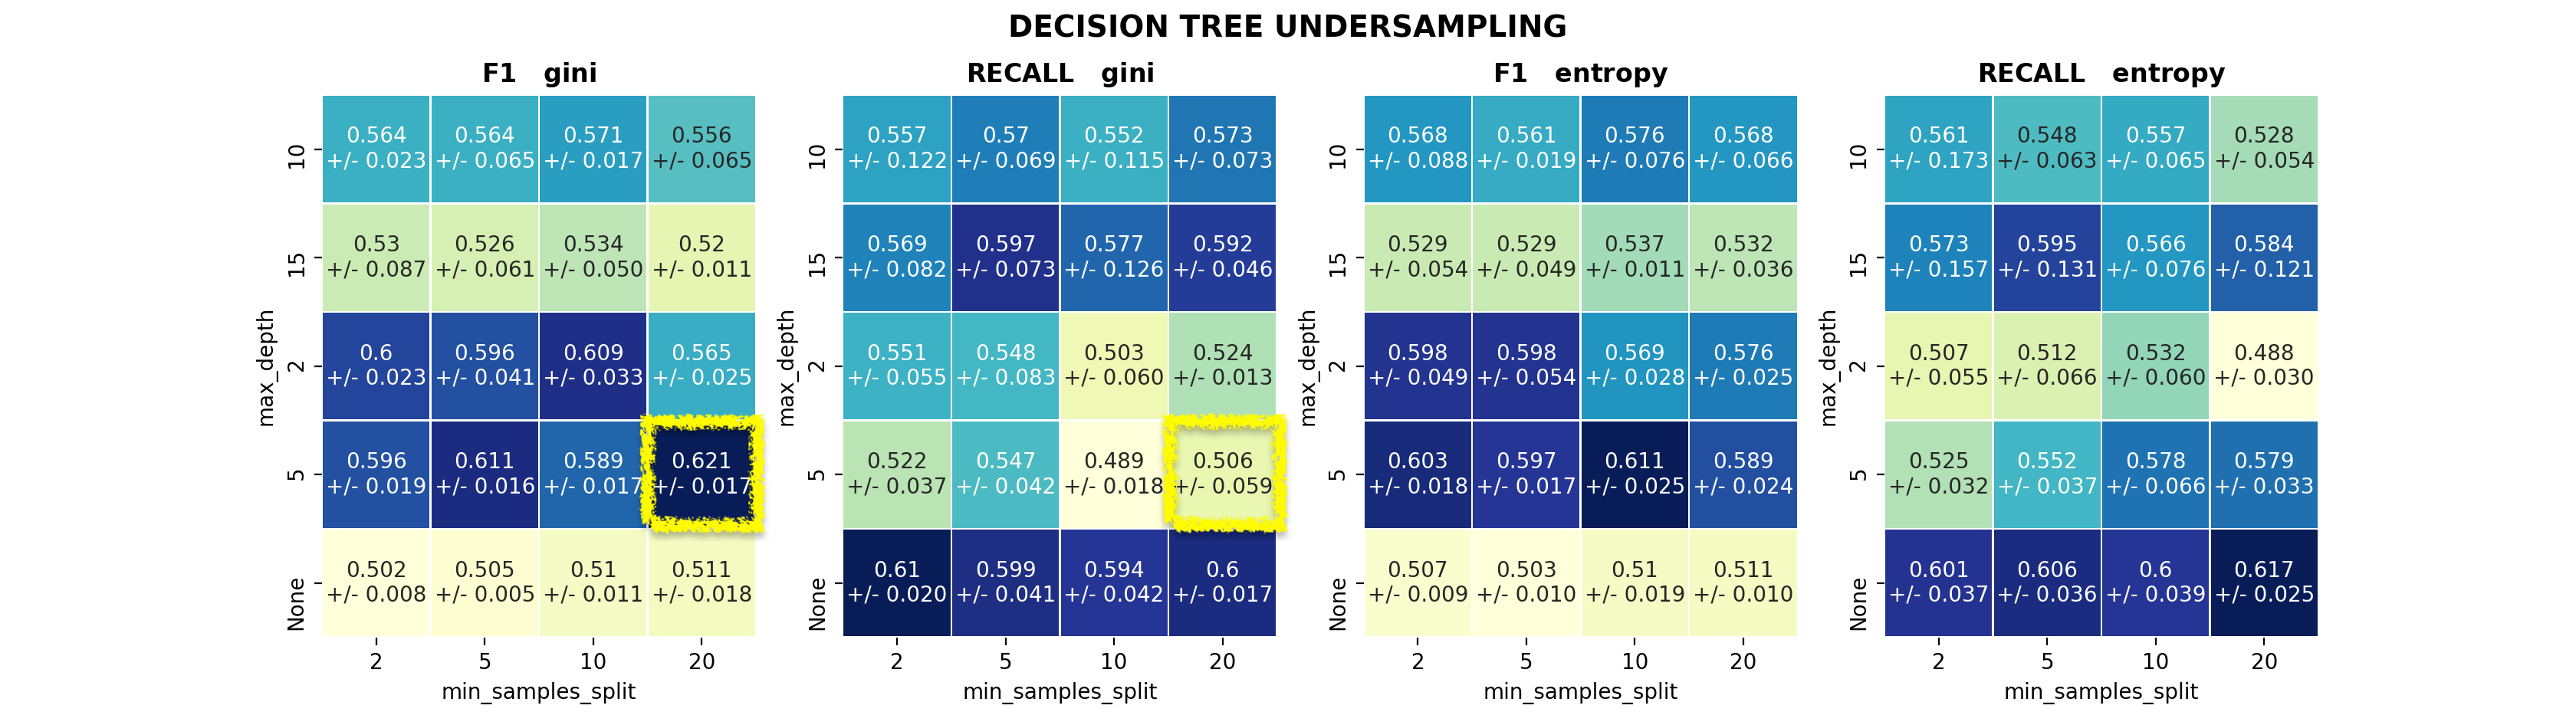
\includegraphics[width=.9\textwidth]{clf_img/DecisionTree_US.png}
		\caption{Decision Tree + Undersampling tuning}
		\label{fig:hyper_dectreeUS}
	\end{figure}
	
	
	\subsubsection{AdaBoost}
	\begin{figure}[H]
		\centering
		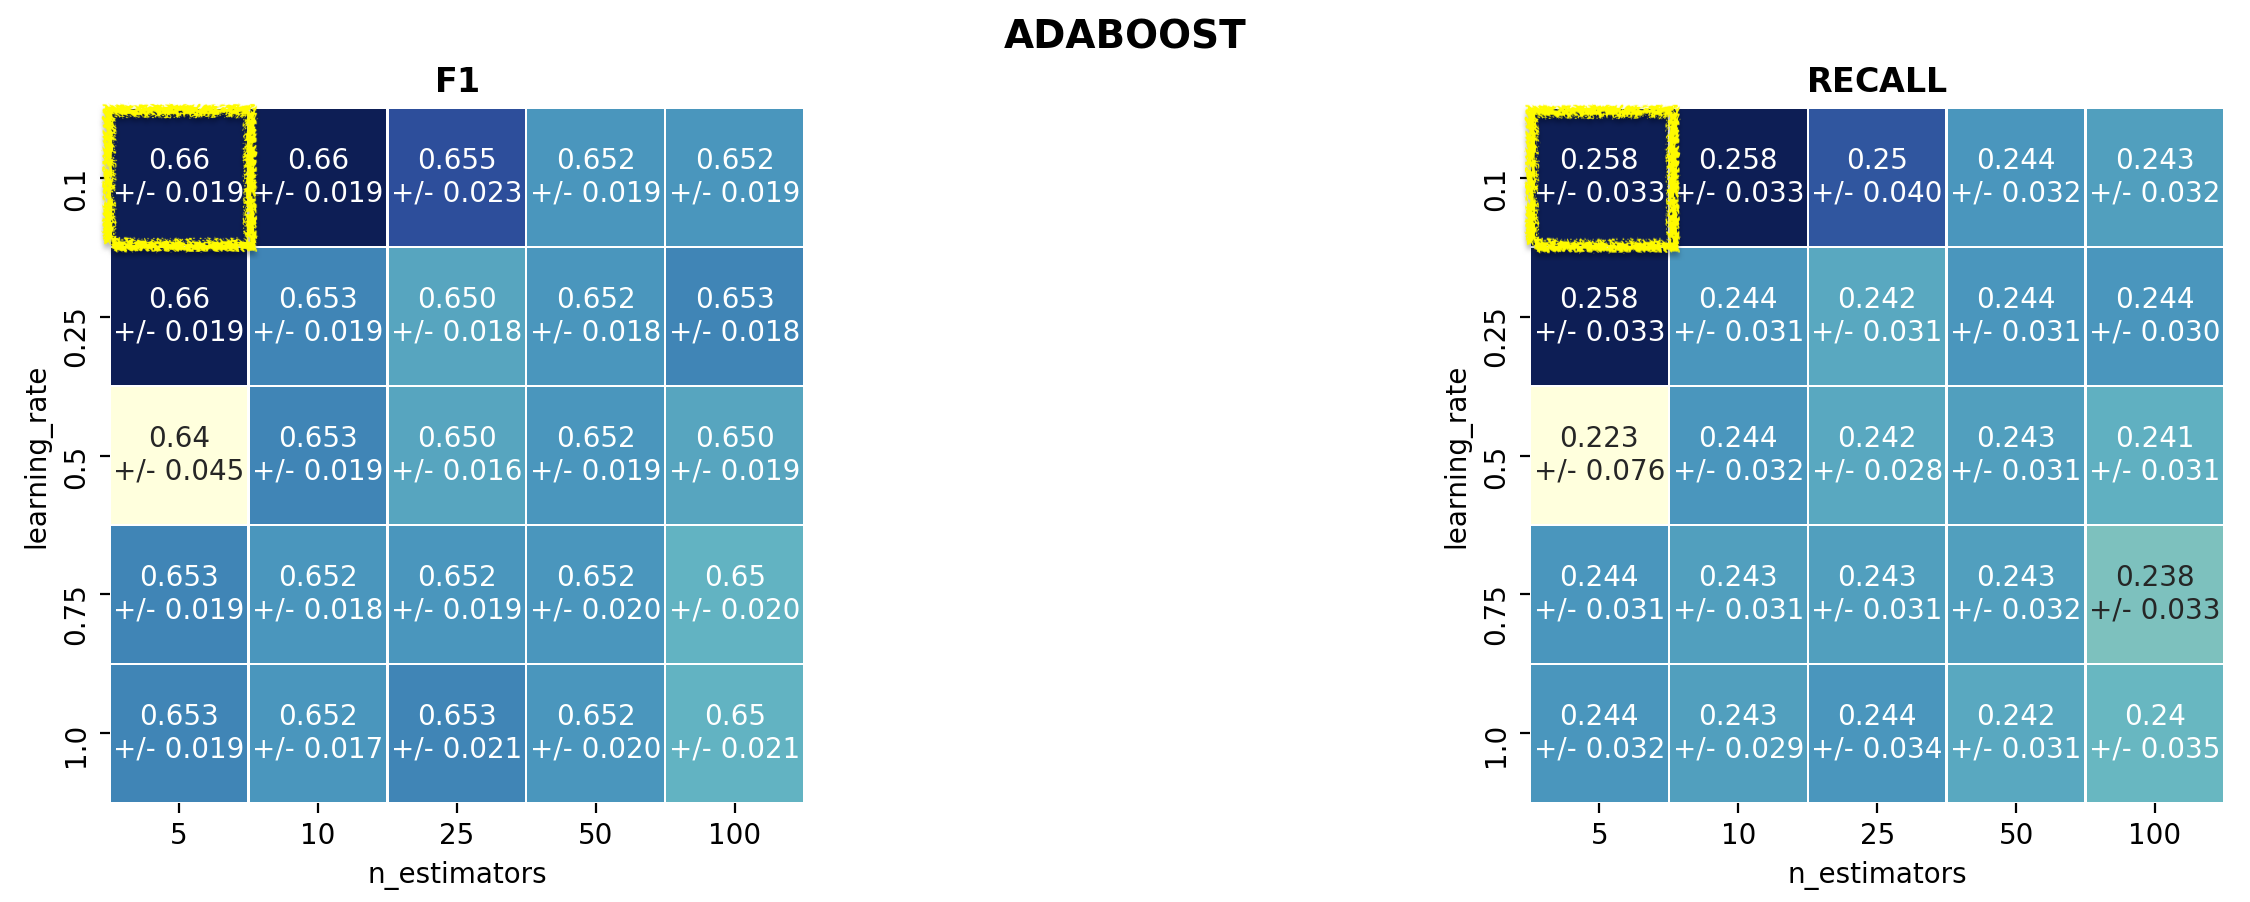
\includegraphics[width=.8\textwidth]{clf_img/Adaboost.png}
		\caption{AdaBoost tuning}
		\label{fig:hyper_ada}
	\end{figure}
	
	\begin{figure}[H]
		\centering
		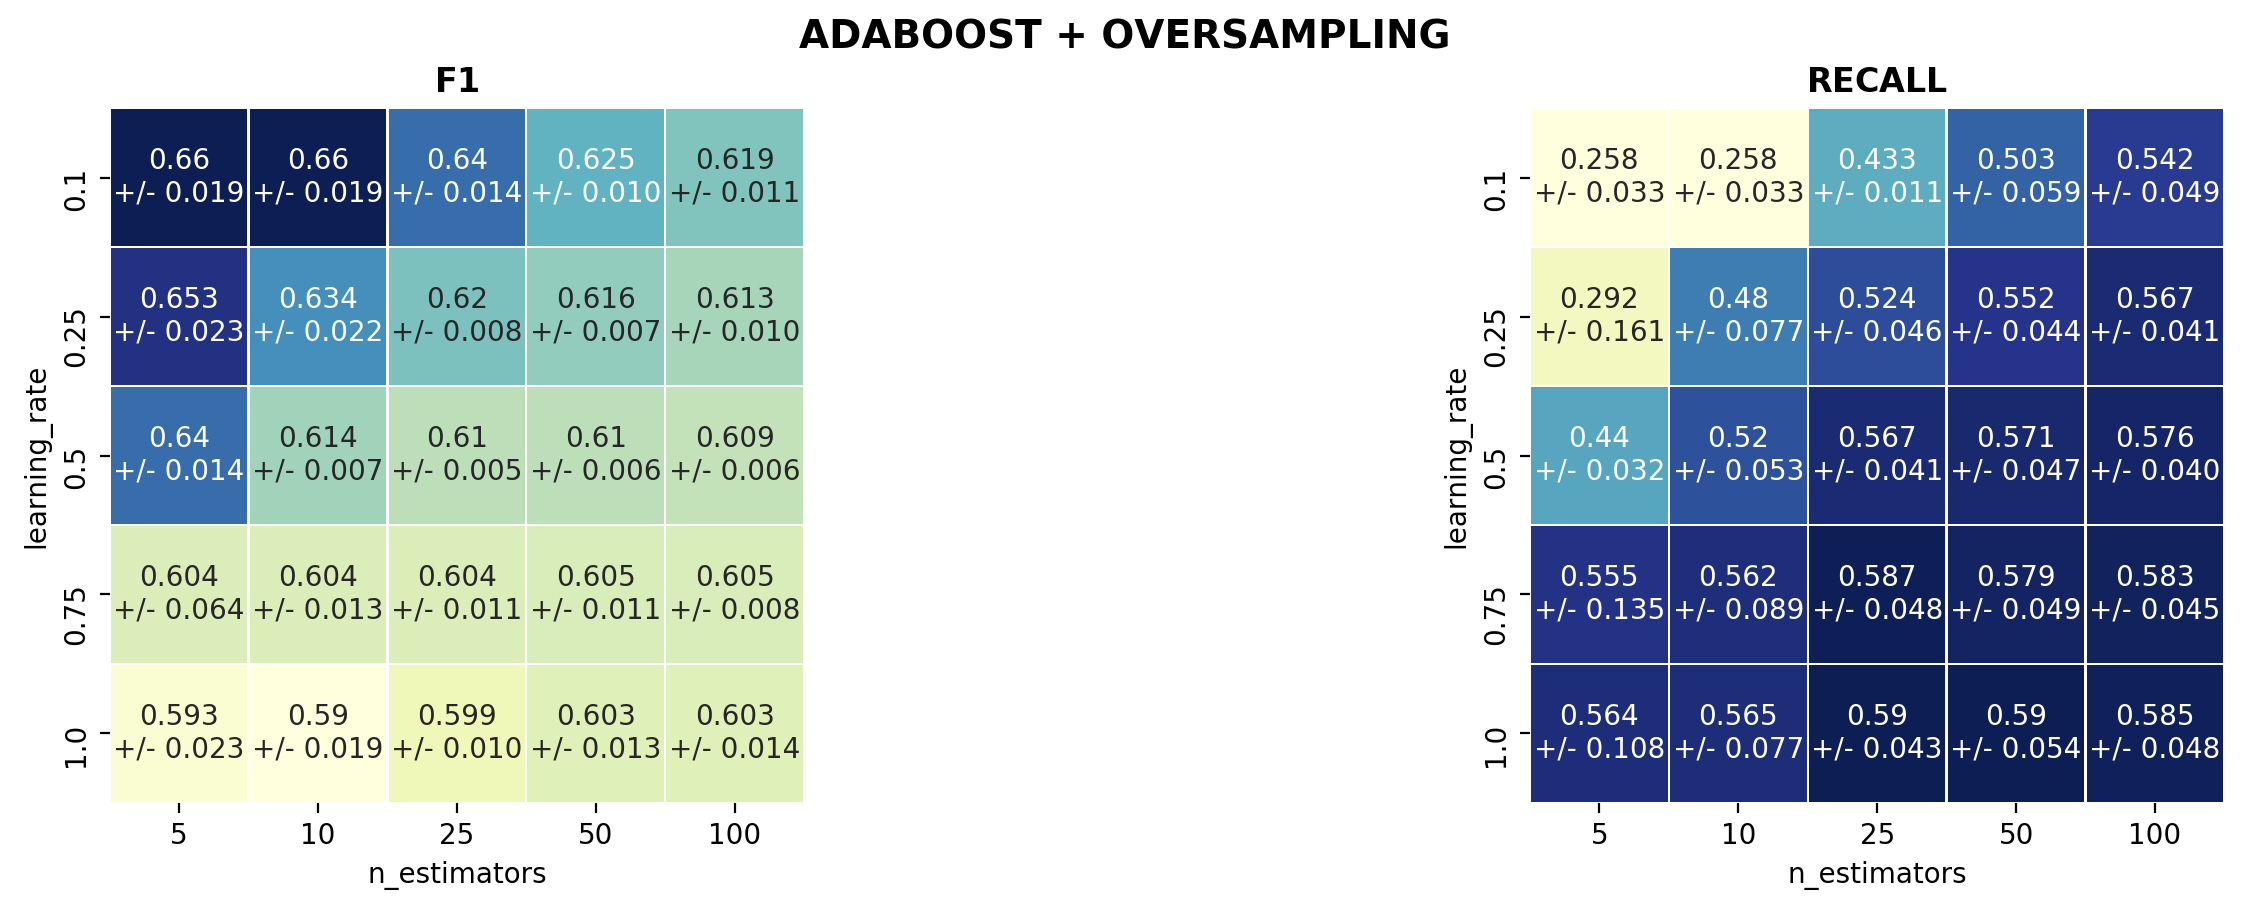
\includegraphics[width=.8\textwidth]{clf_img/Adaboost_OS.png}
		\caption{AdaBoost + Oversampling tuning}
		\label{fig:hyper_adaOS}
	\end{figure}
	
	\begin{figure}[H]
		\centering
		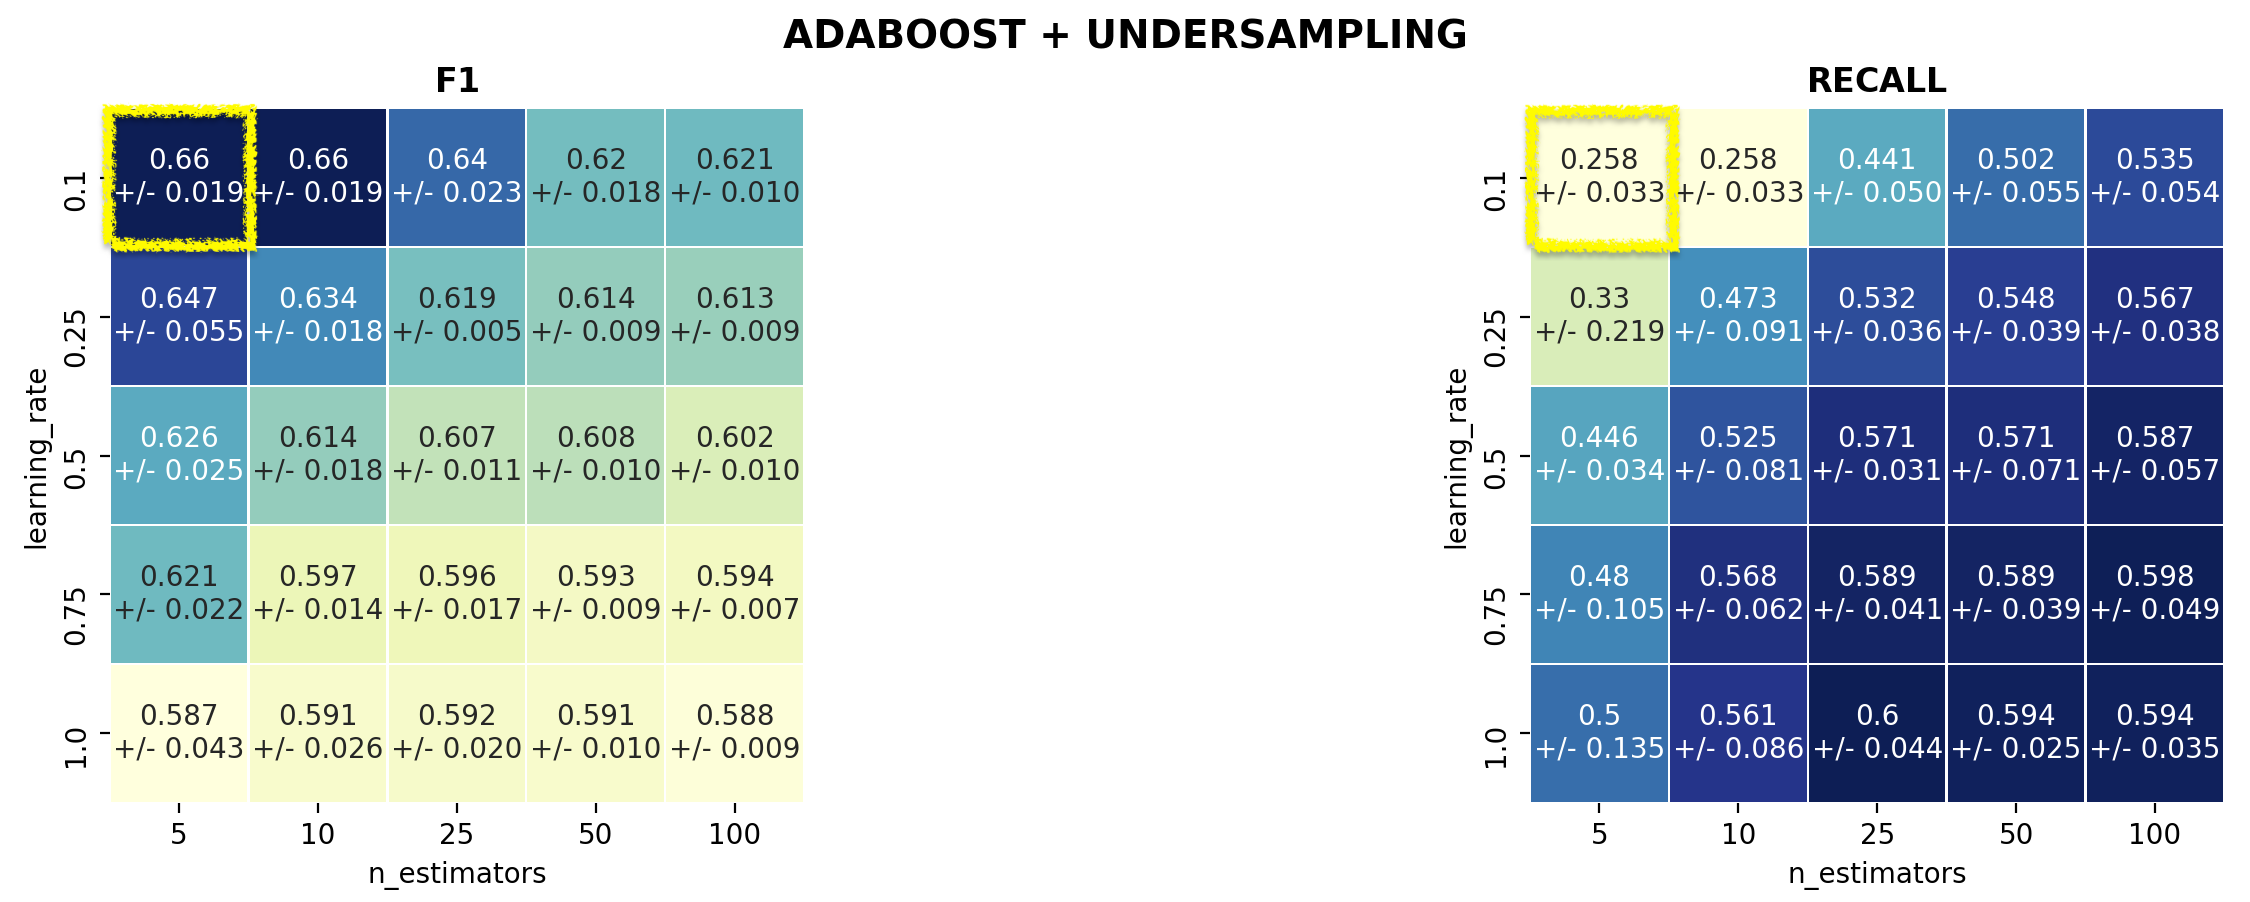
\includegraphics[width=.8\textwidth]{clf_img/Adaboost_US.png}
		\caption{AdaBoost + Undersampling tuning}
		\label{fig:hyper_adaUS}
	\end{figure}
	
	
	\subsection{Optimized Algorithms : Results}
	Once discovered the best settings for each algorithm, we trained those algorithms using their best parameters. As far as the input data concerns, we adopted the whole training set. Afterwards, we verified the performance using the given test set. Table \ref{tab:restest} highlights that the best approach for this task is Random Forest without any class balancing. 
	
	\subsection{Decision Tree interpretation}
	Although the decision tree is not the best method to predict the required variable, its scores are still valid. Note that the following pictures refer to the optimized decision tree that has been trained using a max\_depth equal to 2. The most evident point is that the "WheelType" column owns importance that is more than 80\%. Hence, a row having the "WheelType" attribute equal to "NULL" (greater than 3.5) is a potentially risky affair.
	
	\begin{figure}[H]
		\centering
		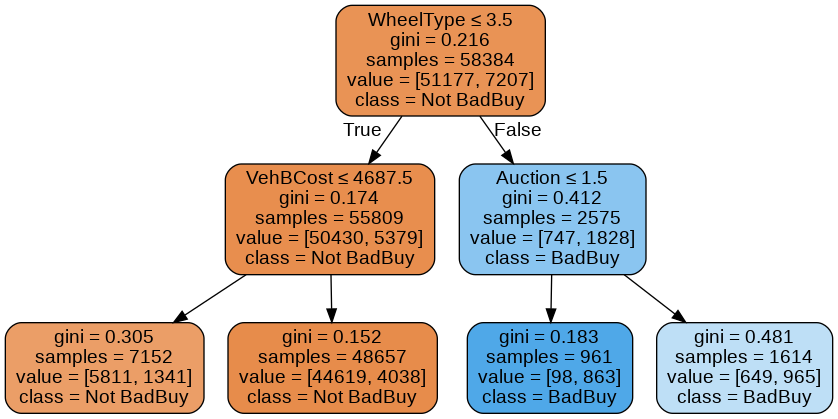
\includegraphics[width=.55\textwidth]{dectree.png}\hfill
		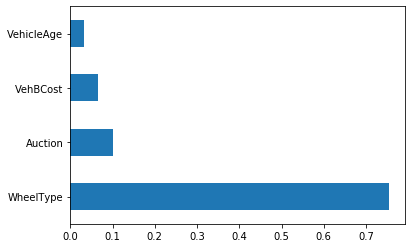
\includegraphics[width=.45\textwidth]{dectreevar.png}\hfill
		\caption{Optimized Decision Tree}
		\label{fig:optdectree}
	\end{figure}
	
	
	
	% Please add the following required packages to your document preamble:
	% \usepackage{multirow}
	% \usepackage[table,xcdraw]{xcolor}
	% If you use beamer only pass "xcolor=table" option, i.e. \documentclass[xcolor=table]{beamer}
	\begin{table}[]
		\begin{tabular}{c|c|c|c|c|c|c|c|c|c|c|}
			\cline{2-11}
			& \cellcolor[HTML]{656565}{\color[HTML]{FFFFFF} }                                    & \multicolumn{3}{c|}{\cellcolor[HTML]{656565}{\color[HTML]{FFFFFF} \textbf{Precision}}}                                                                            & \multicolumn{3}{c|}{\cellcolor[HTML]{656565}{\color[HTML]{FFFFFF} \textbf{Recall}}}                                                                               & \multicolumn{3}{c|}{\cellcolor[HTML]{656565}{\color[HTML]{FFFFFF} \textbf{F1-Score}}}                                                                             \\ \cline{3-11} 
			& \multirow{-2}{*}{\cellcolor[HTML]{656565}{\color[HTML]{FFFFFF} \textbf{Accuracy}}} & \cellcolor[HTML]{9B9B9B}{\color[HTML]{FFFFFF} 0} & \cellcolor[HTML]{9B9B9B}{\color[HTML]{FFFFFF} 1} & \cellcolor[HTML]{9B9B9B}{\color[HTML]{FFFFFF} \textit{AVG}} & \cellcolor[HTML]{9B9B9B}{\color[HTML]{FFFFFF} 0} & \cellcolor[HTML]{9B9B9B}{\color[HTML]{FFFFFF} 1} & \cellcolor[HTML]{9B9B9B}{\color[HTML]{FFFFFF} \textit{AVG}} & \cellcolor[HTML]{9B9B9B}{\color[HTML]{FFFFFF} 0} & \cellcolor[HTML]{9B9B9B}{\color[HTML]{FFFFFF} 1} & \cellcolor[HTML]{9B9B9B}{\color[HTML]{FFFFFF} \textit{AVG}} \\ \hline
			\rowcolor[HTML]{9AFF99} 
			\multicolumn{1}{|c|}{\cellcolor[HTML]{9AFF99}Random Forest}                 & \textbf{0.90}                                                                      & 0.90                                             & 0.81                                             & \textbf{0.85}                                               & 0.99                                             & 0.22                                             & \textbf{0.61}                                               & 0.95                                             & 0.35                                             & \textbf{0.65}                                               \\ \hline
			\rowcolor[HTML]{E6E6E6} 
			\multicolumn{1}{|c|}{\cellcolor[HTML]{E6E6E6}Random Forest + OverSampling}  & \textbf{0.90}                                                                      & 0.90                                             & 0.78                                             & \textbf{0.84}                                               & 0.99                                             & 0.22                                             & \textbf{0.61}                                               & 0.94                                             & 0.35                                             & \textbf{0.65}                                               \\ \hline
			\multicolumn{1}{|c|}{Random Forest + UnderSampling}                         & \textbf{0.74}                                                                      & \cellcolor[HTML]{FFFFFF}0.92                     & 0.24                                             & \textbf{0.58}                                               & 0.76                                             & 0.54                                             & \textbf{0.65}                                               & 0.84                                             & 0.33                                             & \textbf{0.58}                                               \\ \hline
			\rowcolor[HTML]{E6E6E6} 
			\multicolumn{1}{|c|}{\cellcolor[HTML]{E6E6E6}Decision Tree}                 & \textbf{0.89}                                                                      & 0.90                                             & 0.68                                             & \textbf{0.79}                                               & 0.99                                             & 0.23                                             & \textbf{0.61}                                               & 0.94                                             & 0.35                                             & \textbf{0.64}                                               \\ \hline
			\multicolumn{1}{|c|}{Decision Tree + OverSampling}                          & \textbf{0.72}                                                                      & \cellcolor[HTML]{FFFFFF}0.92                     & 0.23                                             & \textbf{0.58}                                               & 0.75                                             & 0.54                                             & \textbf{0.64}                                               & 0.83                                             & 0.32                                             & \textbf{0.57}                                               \\ \hline
			\rowcolor[HTML]{E6E6E6} 
			\multicolumn{1}{|c|}{\cellcolor[HTML]{E6E6E6}Decision Tree + UnderSampling} & \textbf{0.66}                                                                      & 0.92                                             & 0.20                                             & \textbf{0.56}                                               & 0.66                                             & 0.60                                             & \textbf{0.63}                                               & 0.77                                             & 0.30                                             & \textbf{0.54}                                               \\ \hline
			\multicolumn{1}{|c|}{AdaBoost}                                              & \textbf{0.89}                                                                      & 0.90                                             & 0.68                                             & \textbf{0.79}                                               & 0.99                                             & 0.23                                             & \textbf{0.61}                                               & 0.94                                             & 0.35                                             & \textbf{0.64}                                               \\ \hline
			\rowcolor[HTML]{E6E6E6} 
			\multicolumn{1}{|c|}{\cellcolor[HTML]{E6E6E6}AdaBoost + OverSampling}       & \textbf{0.89}                                                                      & 0.90                                             & 0.68                                             & \textbf{0.79}                                               & 0.99                                             & 0.23                                             & \textbf{0.61}                                               & 0.94                                             & 0.35                                             & \textbf{0.64}                                               \\ \hline
			\multicolumn{1}{|c|}{AdaBoost + OverSampling}                               & \textbf{0.89}                                                                      & 0.90                                             & 0.68                                             & \textbf{0.79}                                               & 0.99                                             & 0.23                                             & \textbf{0.61}                                               & 0.94                                             & 0.35                                             & \textbf{0.64}                                               \\ \hline
		\end{tabular}
		\caption{Results of the optimized algorithm over the test set}
		\label{tab:restest}
	\end{table}
	
	
	
	\section{Pattern Mining}
	\label{sec:patternmining}
	In this section we try to find the best pattern and association rules in order to better understand the information hidden in the dataset. 
	
	\subsection{Attribute selection and binning}
	
	At first, we selected the most informative attributes which are: VehicleAge, Make, Model, Trim, Color, WheelType, VehOdo, AAAP, BYRNO, VNST, VehBCost, WarrantyCost.
	\\ We chose to use these attributes because most of them are coherent with the data used in the previous analysis.\\  
	In order to perform a better pattern mining, we discretized the numerical attributes 'VehOdo', 'VehBCost', 'WarrantyCost', 'AAAP', 'VehicleAge and then, we transformed numerical attributes into string.\\
	Formerly we plotted their distribution, and in accordance with the distribution we chose to split the attributes into five range.\\  
	
	\begin{figure}[H]
		\centering
		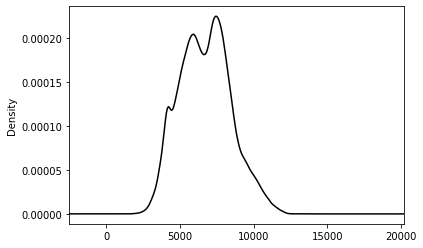
\includegraphics[width=.49\textwidth]{bin1.png}
		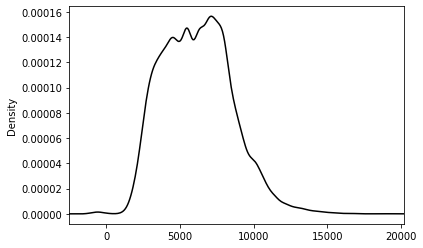
\includegraphics[width=.49\textwidth]{bin2.png}
		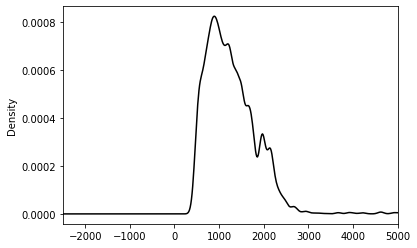
\includegraphics[width=.49\textwidth]{bin3.png}
		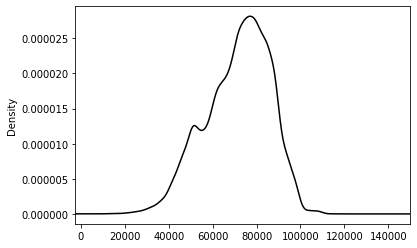
\includegraphics[width=.49\textwidth]{bin4.png}
		\caption{Distribution of numerical attributes}
		\label{fig:hyper_rf}
	\end{figure}
	
	On the top left we bins = [df.VehBCost.min() - 1,5000, 7000, 8000, 10000, df.VehBCost.max()]
	down left bins = [df.WarrantyCost.min() - 1,700, 1200, 1800, 2600, df.WarrantyCost.max()]
	top right bins = [df.AAAP.min() - 1, 3000, 6000, 8000, 10000, df.AAAP.max()]
	right down bins = [df.VehOdo.min() - 1,40000, 60000, 80000, 100000, df.VehOdo.max()]
	
	\subsection{Frequent itemsets extraction}
	
	We ran the Apriori algorithm for frequent itemsets extraction based on the attributes selected. 
	
	\begin{figure}[H]
		\centering
		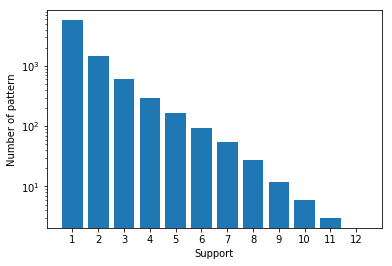
\includegraphics[width=.49\textwidth]{support.png}
		\caption{Frequency plof of itemsets with different value of support}
		\label{fig:hyper_rf_us}
	\end{figure}
	
	\subsubsection{Frequent maximal itemset}
	For frequent  maximal itemsets we used a minsupport equals to eight , selecting only sets that have 3 elements.
	
	\begin{table}[H]
		\centering
		\begin{tabular}{c|ccccccc}
			\hline
			Pattern & Support \\
			\hline
			\rowcolor{Gray}
			'VehBCost:(5000.0, 7000.0]', 'AAAP:(3000.0, 6000.0]', 'Age:[4, 6)') &  6798\\
			'VehBCost:(5000.0, 7000.0]', 'AAAP:(3000.0, 6000.0]', 'Covers') &  6653\\
			\rowcolor{Gray}
			'AAAP:(3000.0, 6000.0]', 'Age:[4, 6)', 'Covers') &  6458\\
			'Age:[4, 6)', 'Odo:(60000, 80000]', 'Alloy') &  6392\\
			\rowcolor{Gray}
			'AAAP:(3000.0, 6000.0]', 'Age:[4, 6)', 'Odo:(60000, 80000]') &  6222\\
			'VehBCost:(5000.0, 7000.0]', 'AAAP:(3000.0, 6000.0]', 'Odo:(60000, 80000]')  & 5936\\
			\rowcolor{Gray}
			'AAAP:(3000.0, 6000.0]', 'Age:[4, 6)', 'Alloy') &  5794\\
			'WarrCost:(1200, 1800]', 'Odo:(60000, 80000]', 'Alloy') & 5641\\
			\rowcolor{Gray}
			'VehBCost:(5000.0, 7000.0]', 'AAAP:(3000.0, 6000.0]', 'Alloy') &  5410\\
			'VehBCost:(5000.0, 7000.0]', 'Covers', 'Odo:(60000, 80000]') & 5373\\
		\end{tabular}
		\caption{Number of maximal itemsets with support equals to 8}
	\end{table}
	
	\subsubsection{Frequent closed itemsets}
	For frequent itemsets we used a minsupport equal to 11\%, selecting only sets that have 3 elements
	
	\begin{table}[H]
		\centering
		\begin{tabular}{c|ccccccc}
			\hline
			Pattern & Support \\
			\hline
			\rowcolor{Gray}
			'VehBCost:(5000.0, 7000.0]', 'AAAP:(3000.0, 6000.0]', 'Age:[4, 6)' & 6798\\
			(('VehBCost:(5000.0, 7000.0]', 'AAAP:(3000.0, 6000.0]', 'Covers' & 6653\\
			\rowcolor{Gray}
			(('AAAP:(3000.0, 6000.0]', 'Age:[4, 6)', 'Covers' &  6458\\
			(('Age:[4, 6)', 'Odo:(60000, 80000]', 'Alloy' &  6392\\
			\rowcolor{Gray}
			(('AAAP:(3000.0, 6000.0]', 'Age:[4, 6)', 'Odo:(60000, 80000]' &  6222\\
			(('VehBCost:(5000.0, 7000.0]', 'AAAP:(3000.0, 6000.0]', 'Odo:(60000, 80000]' & 5936\\
		\end{tabular}
		\caption{Number of closed itemsets with support equals to 10}
	\end{table}
	
	\subsubsection{Frequent itemsets}
	
	For frequent itemsets we used a minsupport equal to 30\% ,selecting only sets that have 3 elements. The list of the frequent itemsets is largely the same with the closed ones, because the  it is a superset of the latter one. (DA RISCRIVERE). 
	
	\begin{table}[H]
		\centering
		\begin{tabular}{c|ccccccc}
			\hline
			Pattern & Support \\
			\hline
			\rowcolor{Gray}
			'VehBCost:(5000.0, 7000.0]', 'AAAP:(3000.0, 6000.0]',  'Age:[4, 6)') & 6798 \\
			'VehBCost:(5000.0, 7000.0]', 'AAAP:(3000.0, 6000.0]' ,  'Covers'  & 6653 \\
			\rowcolor{Gray}
			'AAAP:(3000.0, 6000.0]', 'Age:[4, 6)', 'Covers' & 6458) \\
		\end{tabular}
		\caption{Number of maximal itemsets with support equals to 11}
	\end{table}
	
	\subsection{Association Rules}
	In this section we discuss the most interesting association rules obtained with the Apriori algorithm. 
	We decided to extract these rules considering only the frequent itemsets with a length major or equal to 3. 
	The association rules are shown in the following tables.  
	
	\subsubsection{Association Rules for missing value replacement}
	
	Given the frequent itemetes founds in Section, we decided to use the rules that best represent car's auction.\\
	For this reason, we use the rules characterized by greater support and best lift value.
	
	
	\begin{table}[H]
		\centering
		\begin{tabular}{|cc|cc|}
			\hline
			\textbf{RHS} & \textbf{LHS} & \textbf{Confidence} & \textbf{Lift} \\
			\hline
			\rowcolor{Gray}
			Alloy & FORD  & 0.767 & 1.523 \\
			Covers & Age:[2, 4)', 'VehBCost:(5000.0, 7000.0]  & 0.687 & 1.501 \\
			\rowcolor{Gray}
			Alloy &  ('Odo:(80000, 100000]', 'WarrCost:(1200, 1800]') &  0.678 & 1.346 \\
			\hline
		\end{tabular}
		\caption{Most significant association rules for missing value replacement}
	\end{table}
	
	
	
	
	
	\subsubsection{Association Rules for predicting target variable}
	To predict the target variable we decided to generate a new data set in order to balance the number of 'badbuy' and 'goodbuy' with the aim to produce not only association rules for 'goodbuy', which are the majority of attributes, but also for 'badbuy'.\\
	We selected the most significant rules  by using support equals to 10 and confidence of 0.67 and then, we selected rules with  a higher confidence and lift as we can see in the Table 8.\\
	By using these rules we try to predict the target variable in the data set obtaining the 83\% of accuracy.\\
	
	\begin{figure}[H]
		\centering
		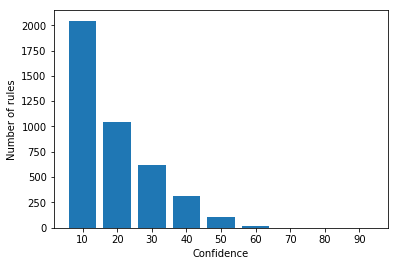
\includegraphics[width=.49\textwidth]{rules.png}
		\caption{Frequency plof of rules with different value of confidence}
		\label{fig:hyper_rf_us}
	\end{figure}
	
	
	
	
	\begin{table}[H]
		\centering
		\begin{tabular}{|cc|cc|}
			\hline
			\textbf{RHS} & \textbf{LHS} & \textbf{Confidence} & \textbf{Lift} \\
			\hline
			\rowcolor{Gray}
			GoodBuy & AAAP:(6000.0, 8000.0], Covers'  & 0.701 & 1.402 \\
			GoodBuy & Age:[2, 4), Covers' & 0.686 & 1.373 \\
			\rowcolor{Gray}
			GoodBuy &  CHRYSLER, Covers &  0.647 & 1.295 \\
			BadBuy &  VehBCost:(224.0, 5000.0], AAAP:(3000.0, 6000.0] & 0.613 & 1.226\\
			\hline
		\end{tabular}
		\caption{Most significant association rules for prediction the target variable}
	\end{table}
	
	\begin{table}[H]
		\centering
		\begin{tabular}{cc|cc}
			\multicolumn{1}{c}{} &\multicolumn{1}{c}{} &\multicolumn{1}{c}{\textbf{Predicted Value}} \\ 
			\multicolumn{1}{c}{} & 
			\multicolumn{1}{c|}{} & 
			\multicolumn{1}{c}{\textbf{GoodBuy}} & 
			\multicolumn{1}{c}{\textbf{BadBuy}} \\ \hline
			\multirow{2}{*}{\rotatebox{1}{\textbf{Actual Value}}}
			& \textbf{GoodBuy}  & 47548 & 3629   \\ 
			& \textbf{BadBuy}  & 6295  & 912 \\ \hline
		\end{tabular}
		\caption{Confusion matrix obtained from the application of the association rulss for the target variable prediction }
	\end{table}
	
	
	
	
	
	
	\section{Conclusion}
	
	Chi ha tolto il cafféééééééé???
	
	
\end{document}


